% Default language option is [thaithesis]. The other possible option is [engthesis].
% Default format option is [ugrad]. Other possible options are [master,doctor].
%\documentclass[a4paper]{chula-memoir}
%\documentclass[a4paper,thaithesis,master]{chula-memoir}
\documentclass[a4paper,engthesis,master]{chula-memoir}


\usepackage{ulem}
% List all required packages here
\usepackage{float}              % for floating figures
\usepackage{amsmath}            % for math related environment
\usepackage{amsfonts}           % fonts for math
\usepackage{listings}           % for pseudo-code, lines of codes
\usepackage[labelformat=simple]{subcaption}
\renewcommand\thesubfigure{(\alph{subfigure})}    % for (a) in subcaption
\usepackage{enumitem}
\usepackage{graphicx}
\usepackage{wrapfig}            % for figures wrap inside text paragraph
\usepackage{pdfpages}           % for including pdf pages
\usepackage{verbatim}           % for block comment
\usepackage{multicol}

\usepackage{standalone}         % for proposal text inclusion
\usepackage{pgfgantt}           % for gantt chart
\usepackage{longtable}          % for multi-page table



\usepackage{amsthm}
\usepackage{enumitem}
\usepackage{amssymb}

\usepackage{tikz}










\newtheorem{theorem}{Theorem}[section]
\newtheorem{corollary}[theorem]{Collorary}
\newtheorem{lemma}[theorem]{Lemma}
\newtheorem{note}[theorem]{Note}

\theoremstyle{definition}
\newtheorem{definition}[theorem]{Definition}
\newtheorem{fact}[theorem]{Fact}
\newtheorem{remark}[theorem]{Remark}
\newtheorem{conjecture}[theorem]{Conjecture}
\usepackage{hyperref}


\renewcommand{\restriction}{\mathord{\upharpoonright}}
\newcommand{\mdot}{\cdot\cdot\cdot}
\newcommand{\seq}{\textup{seq}}
\newcommand{\fin}{\textup{fin}}
\newcommand{\fix}{\textup{fix}}
\newcommand{\m}{\textup{m}}
\newcommand{\ran}{\textup{ran}}
\newcommand{\dom}{\textup{dom}}
\renewcommand{\max}{\textup{max}}

\newcommand{\quotate}[1]{\lq\lq{#1}\rq\rq} %``
\renewcommand{\frak}{\mathfrak}
\newcommand{\mcal}{\mathcal}
\newcommand{\sym}{\textup{sym}}






% listings format
\lstset{
basicstyle=\ttfamily,
numbers=left,
numberstyle=\small,
xleftmargin=.1\linewidth,
frame=single,
captionpos=b,
columns=fullflexible,
breaklines=true,
keepspaces=true,
showstringspaces=false,
}

\usepackage{tikz}
\usetikzlibrary{shapes,positioning,arrows,backgrounds,fit,decorations.pathreplacing}
\usepackage{adjustbox}
\usepackage[ruled,vlined]{algorithm2e}


% \setlength{\arrayrulewidth}{1mm}
\setlength{\tabcolsep}{10pt}
\newcolumntype{C}[1]{>{\centering\let\newline\\\arraybackslash\hspace{0pt}}m{#1}}

%% helper commands
\newcommand\Tstrut{\rule{0pt}{2.6ex}}         % = `top' strut
\newcommand\Bstrut{\rule[-0.9ex]{0pt}{0pt}}   % = `bottom' strut

\newbox\mybox
\def\centerfigureone#1{%
    \setbox\mybox\hbox{#1}%
    \raisebox{-0.3\dimexpr\ht\mybox+\dp\mybox}{\copy\mybox}%
}

\newbox\mybox
\def\centerfiguretwo#1{%
    \setbox\mybox\hbox{#1}%
    \raisebox{-0.4\dimexpr\ht\mybox+\dp\mybox}{\copy\mybox}%
}

\newbox\mybox
\def\centerfigurethree#1{%
    \setbox\mybox\hbox{#1}%
    \raisebox{-0.4\dimexpr\ht\mybox+\dp\mybox}{\copy\mybox}%
}

%% Quantum related commands
\newcommand{\ket}[1]{\ensuremath{\left|#1\right\rangle}} % Dirac Kets

\newcommand{\qgate}[1]{
    \centerfigureone{
        \begin{tikzpicture}[thick]
        %
        % `operator' will only be used by Hadamard (H) gates here.
        % `phase' is used for controlled phase gates (dots).
        % `surround' is used for the background box.
        \tikzstyle{operator} = [draw,fill=white,minimum size=1.5em] 
        \tikzstyle{phase} = [fill,shape=circle,minimum size=5pt,inner sep=0pt]
        \tikzstyle{surround} = [fill=blue!10,thick,draw=black,rounded corners=2mm]
        %
        % Qubits
        \node at (0,0) (q1) {};
        %
        % Column 1
        \node[operator] (op11) at (1,0) {#1} edge [-] (q1);
        %
        % Column 6
        \node (end1) at (2,0) {} edge [-] (op11);
        %
    \end{tikzpicture}
    }
}

%% two params
%% first param - choose the symbol of controlled gate
%% second param - letter for the gate is any
\newcommand{\qcontrolgate}[2]{
    \centerfiguretwo{
        \begin{tikzpicture}[thick]
            %
            % `operator' will only be used by Hadamard (H) gates here.
            % `phase' is used for controlled phase gates (dots).
            % `surround' is used for the background box.
            % `crossx' is used for the cross.
            % `circlewc' is used for the circle with cross box.
            \tikzstyle{operator} = [draw,fill=white,minimum size=1.5em] 
            \tikzstyle{phase} = [fill,shape=circle,minimum size=5pt,inner sep=0pt]
            \tikzstyle{surround} = [fill=blue!10,thick,draw=black,rounded corners=2mm]
            \tikzstyle{circlewc} = [draw,circle,cross,minimum width=0.3 cm]
            \tikzstyle{cross} = [path picture={ 
                \draw[thick,black](path picture bounding box.north) -- (path picture bounding box.south) (path picture bounding box.west) -- (path picture bounding box.east);
                }]
            \tikzstyle{crossx} = [path picture={ 
                \draw[thick,black,inner sep=0pt]
                (path picture bounding box.south east) -- (path picture bounding box.north west) (path picture bounding box.south west) -- (path picture bounding box.north east);
                }]
            %
            % Qubits
            \node at (0,0) (q1) {};
            \node at (0,-1) (q2) {};
            %
            % Column 1
            \node[phase] (phase11) at (1,0) {} edge [-] (q1);
            \node[#1] (cw12) at (1,-1) {#2} edge [-] (q2);
            \draw[-] (phase11) -- (cw12);
            %
            % Column 2
            \node (end1) at (2,0) {} edge [-] (phase11);
            \node (end2) at (2,-1) {} edge [-] (cw12);
        \end{tikzpicture}
    }
}

\newcommand{\swapgate}{
    \centerfiguretwo{
        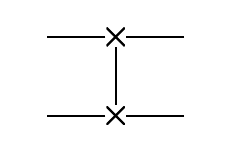
\begin{tikzpicture}[thick]
            %
            % `operator' will only be used by Hadamard (H) gates here.
            % `phase' is used for controlled phase gates (dots).
            % `surround' is used for the background box.
            % `crossx' is used for the cross.
            % `circlewc' is used for the circle with cross box.
            \tikzstyle{operator} = [draw,fill=white,minimum size=1.5em] 
            \tikzstyle{phase} = [fill,shape=circle,minimum size=5pt,inner sep=0pt]
            \tikzstyle{surround} = [fill=blue!10,thick,draw=black,rounded corners=2mm]
            \tikzstyle{circlewc} = [draw,circle,cross,minimum width=0.3 cm]
            \tikzstyle{cross} = [path picture={ 
                \draw[thick,black](path picture bounding box.north) -- (path picture bounding box.south) (path picture bounding box.west) -- (path picture bounding box.east);
                }]
            \tikzstyle{crossx} = [path picture={ 
                \draw[thick,black,inner sep=0pt]
                (path picture bounding box.south east) -- (path picture bounding box.north west) (path picture bounding box.south west) -- (path picture bounding box.north east);
                }]
            %
            % Qubits
            \node at (0,0) (q1) {};
            \node at (0,-1) (q2) {};
            %
            % Column 1
            \node[crossx] (phase11) at (1,0) {} edge [-] (q1);
            \node[crossx] (cw12) at (1,-1) {} edge [-] (q2);
            \draw[-] (phase11) -- (cw12);
            %
            % Column 2
            \node (end1) at (2,0) {} edge [-] (phase11);
            \node (end2) at (2,-1) {} edge [-] (cw12);
        \end{tikzpicture}
    }
}

\newcommand{\toffoligate}{
    \centerfigurethree{
        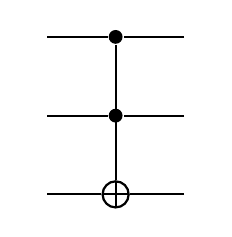
\begin{tikzpicture}[thick]
            %
            % `operator' will only be used by Hadamard (H) gates here.
            % `phase' is used for controlled phase gates (dots).
            % `surround' is used for the background box.
            % `crossx' is used for the cross.
            % `circlewc' is used for the circle with cross box.
            \tikzstyle{operator} = [draw,fill=white,minimum size=1.5em] 
            \tikzstyle{phase} = [fill,shape=circle,minimum size=5pt,inner sep=0pt]
            \tikzstyle{surround} = [fill=blue!10,thick,draw=black,rounded corners=2mm]
            \tikzstyle{circlewc} = [draw,circle,cross,minimum width=0.3 cm]
            \tikzstyle{cross} = [path picture={ 
                \draw[thick,black](path picture bounding box.north) -- (path picture bounding box.south) (path picture bounding box.west) -- (path picture bounding box.east);
                }]
            \tikzstyle{crossx} = [path picture={ 
                \draw[thick,black,inner sep=0pt]
                (path picture bounding box.south east) -- (path picture bounding box.north west) (path picture bounding box.south west) -- (path picture bounding box.north east);
                }]
            %
            % Qubits
            \node at (0,0) (q1) {};
            \node at (0,-1) (q2) {};
            \node at (0,-2) (q3) {};
            %
            % Column 1
            \node[phase] (phase11) at (1,0) {} edge [-] (q1);
            \node[phase] (phase21) at (1,-1) {} edge [-] (q2);
            \node[circlewc] (cw31) at (1,-2) {} edge [-] (q3);
            \draw[-] (phase11) -- (cw31);
            %
            % Column 2
            \node (end1) at (2,0) {} edge [-] (phase11);
            \node (end2) at (2,-1) {} edge [-] (phase21);
            \node (end3) at (2,-2) {} edge [-] (cw31);
        \end{tikzpicture}
    }
}

\newcommand{\measurementgate}{
    \centerfigureone{
        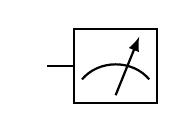
\begin{tikzpicture}[thick]
        %
        % `operator' will only be used by Hadamard (H) gates here.
        % `phase' is used for controlled phase gates (dots).
        % `surround' is used for the background box.
        \tikzstyle{operator} = [draw,fill=white,minimum size=1.5em] 
        \tikzstyle{phase} = [fill,shape=circle,minimum size=5pt,inner sep=0pt]
        \tikzstyle{surround} = [fill=blue!10,thick,draw=black,rounded corners=2mm]
        \tikzset{meter/.append style={draw, inner sep=10, rectangle, font=\vphantom{A}, minimum width=30, line width=.8,
             path picture={\draw[black] ([shift={(.1,.3)}]path picture bounding box.south west) to[bend left=50] ([shift={(-.1,.3)}]path picture bounding box.south east);\draw[black,-latex] ([shift={(0,.1)}]path picture bounding box.south) -- ([shift={(.3,-.1)}]path picture bounding box.north);}}}
        %
        % Qubits
        \node at (0,0) (q1) {};
        %
        % Column 1
        \node[meter] (op11) at (1,0) {} edge [-] (q1);
        %
    \end{tikzpicture}
    }
}

\newcommand{\qubitwire}{
    \centerfigureone{
        \begin{tikzpicture}[thick]
        %
        % `operator' will only be used by Hadamard (H) gates here.
        % `phase' is used for controlled phase gates (dots).
        % `surround' is used for the background box.
        \tikzstyle{operator} = [draw,fill=white,minimum size=1.5em] 
        \tikzstyle{phase} = [fill,shape=circle,minimum size=5pt,inner sep=0pt]
        \tikzstyle{surround} = [fill=blue!10,thick,draw=black,rounded corners=2mm]
        \tikzset{meter/.append style={draw, inner sep=10, rectangle, font=\vphantom{A}, minimum width=30, line width=.8,
             path picture={\draw[black] ([shift={(.1,.3)}]path picture bounding box.south west) to[bend left=50] ([shift={(-.1,.3)}]path picture bounding box.south east);\draw[black,-latex] ([shift={(0,.1)}]path picture bounding box.south) -- ([shift={(.3,-.1)}]path picture bounding box.north);}}}
        %
        % Qubits
        \node at (0,0) (q1) {};
        %
        % Column 1
        \node (op11) at (2,0) {} edge [-] (q1);
        %
        \end{tikzpicture}
    }
}

\newcommand{\classicalwire}{
    \centerfigureone{
        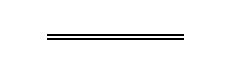
\begin{tikzpicture}[thick]
        %
        % `operator' will only be used by Hadamard (H) gates here.
        % `phase' is used for controlled phase gates (dots).
        % `surround' is used for the background box.
        \tikzstyle{operator} = [draw,fill=white,minimum size=1.5em] 
        \tikzstyle{phase} = [fill,shape=circle,minimum size=5pt,inner sep=0pt]
        \tikzstyle{surround} = [fill=blue!10,thick,draw=black,rounded corners=2mm]
        \tikzset{meter/.append style={draw, inner sep=10, rectangle, font=\vphantom{A}, minimum width=30, line width=.8,
             path picture={\draw[black] ([shift={(.1,.3)}]path picture bounding box.south west) to[bend left=50] ([shift={(-.1,.3)}]path picture bounding box.south east);\draw[black,-latex] ([shift={(0,.1)}]path picture bounding box.south) -- ([shift={(.3,-.1)}]path picture bounding box.north);}}}
        %
        % Qubits
        \node at (0,0) (q1) {};
        %
        % Column 1
        \node (op11) at (2,0) {} edge[double] [-] (q1);
        %
        \end{tikzpicture}
    }
}



%%------------------------------------------------------------
%%-               SETTING THESIS PARAMETERS                  -
%%------------------------------------------------------------

%%------------------------------------------------------------
%%-               SETTING THESIS PARAMETERS                  -
%%------------------------------------------------------------

% set the thesis tile (use {\wbr} for word break)
\thesistitle
% Thai Title
{จำนวนเชิงการนับของเซตของฟังก์ชันหนึ่งต่อหนึ่งและเซตของฟังก์ชันทั่วถึงบนเซต}
% English title (auto upper case)
{CARDINALITIES OF THE SET OF INJECTIONS AND THE SET OF SURJECTIONS ON A SET}

% set the title of the author, e.g., Mr., Miss, Dr. etc.
\authortitle   
% Thai Title of the author                         
{นาย}
% English Title of the author
{Mr.}

% set the author name (must not include title (Mr., Miss, Dr., etc.)
\thesisauthor
% Author name in Thai
{ณัฐจักขณ์ คำกรุ}
% Author name in English
{Natthajak Kamkru}

% set the advisor
\advisor
% Advisor name in Thai
{ผู้ช่วยศาสตราจารย์ ดร. ณัฐพล สนพะเนาว์}
% Advisor name in Thai with abbrev. title
{ผศ. ดร. ณัฐพล สนพะเนาว์}
% Advisor name in English
{Assistant Professor Nattapon Sonpanow, Ph.D.}
% Advisor name in English with abbrev. title (Capital letters except Ph.D.)
{ASST.PROF. NATTAPON SONPANOW, Ph.D.}

% set the faculty
\faculty
% name of the faculty in Thai
{วิทยาศาสตร์}
% name of the faculty in English
{Science}

% set the department
\begin{hyphenrules}{thai}
    \hyphenation{คณิตศาสต์}
\end{hyphenrules}
\department                             
% name of the department in Thai
{คณิตศาสตร์และวิทยาการคอมพิวเตอร์}
% name of the department in English      
{Mathematics and Computer Science}

% set the field of study (สาขาวิชา)
\fieldofstudy
% Field in Thai
{คณิตศาสตร์}
%{คณิตศาสตร์}
% Field in English
{Mathematics}

% set the degree name
\degree
% Degree name in Thai
{วิทยาศาสตรมหาบัณฑิต}                   
% Degree name in English
{ Master of Science}

% Academic Year (in Thai Calendar)
\academicyear{2566}

% ID of the author
\authorid{6570047223}

% Course ID for undergrad report
\subjID{2301499}
% course name
\subjName
% course name in Thai
{โครงงานวิทยาศาสตร์}
% course name in English
{Senior project}


% Keywords, for English abstract
\keywords
{Cardinal, Injection, Surjection}

% name of the dean or department head
\deanname
% in Thai
{ศาสตราจารย์ ดร.ประณัฐ โพธิยะราช}
% in English
{Professor Pranut Potiyaraj, Ph.D.}

% Committee Block
% Specify chair/committee/external committee in your selected language
% list of committee
\committee
{
    % chairman for grad only
    \CommitteeBlock{Chairman}{Professor Pimpen Vejjajiva, Ph.D.}
    % \CommitteeBlock{ประธาน}{ผู้ช่วยศาสตราจารย์ ดร. สมชาย ประสิทธิ์จูตระกูล}

    % pre-defined value for advisor
    \CommitteeBlockAdvisor
    % pre-defined value for co-advisor
    \CommitteeBlockCoAdvisor

 \CommitteeBlock{Committee}{Associate Professor Athipat Thamrongthanyalak, Ph.D.} 
 


    %% กรรมการ
    %\CommitteeBlock{กรรมการ}{อาจารย์ ดร.เพชรอาภา บุญเสริม
     \CommitteeBlock{External Examiner}{Assistant Professor Supakun Panasawatwong, Ph.D.}

   
    %% examiner
    %\CommitteeBlock{Examiner}{Petarpa Boonserm, Ph.D.}

    %% กรรมการภายนอก
    %\CommitteeBlock{กรรมการภายนอก}{ศาสตราจารย์ ดร. ณรงค์ ปั้นนิ่ม} % กรรมการภายนอก

    %% external examiner
    

    % \CommitteeBlock{Examiner}{Petarpa Boonserm, Ph.D.}
    % \CommitteeBlock{กรรมการ}{อาจารย์ ดร.มนนัทธ์ พงษ์พานิช} % examiner
}

\setcitestyle{square}
%%-------------------------------------------------------------------------------
%%-                               DOCUMENT                  -
%%-------------------------------------------------------------------------------
\begin{document}
\frontmatter
% Thesis starts with Thai Cover
\makethaicover
\clearpage



% Followed by English Cover
\makeenglishcover
\clearpage

% Generate committee page
\makecommittee
\clearpage
% Thai Abstract Section
\begin{thaiabstract}
ในปี\hspace{0.15cm}ค.ศ.\hspace{0.1cm}1976\hspace{0.2cm}ดอว์สันและโฮวาร์ดได้แสดงว่าเซตของฟังก์ชันหนึ่งต่อหนึ่งทั่วถึงบนเซต $A$ เขียนแทนด้วย $S(A)$ มีขนาดเท่ากับเซตกำลังของ $A$ เขียนแทนด้วย $\mathcal{P}(A)$ เมื่อ $A$ เป็นเซตอนันต์ ในทฤษฎีเซตแซร์เมโล-แฟรงเคล (ZF) ที่มีสัจพจน์การเลือก (AC) แต่หากปราศจาก AC แล้ว จะไม่สามารถสรุปความสัมพันธ์ระหว่างขนาดของ $S(A)$ และ $\mathcal{P}(A)$ ได้สำหรับเซตอนันต์ $A$ ใด ๆ ต่อมาได้มีการศึกษาความสัมพันธ์ของ $|S(A)|$ กับจำนวนเชิงการนับอื่น ๆ เช่นกัน อาทิ ได้มีการแสดงว่า ``$|\seq(A)|\neq|S(A)|\neq|\seq^{1-1}(A)|$ สำหรับเซตอนันต์ $A$ ใด ๆ" เป็นผลลัพธ์ที่ดีที่สุดใน ZF ที่ปราศจาก AC โดยที่ $\seq(A)$ และ $\seq^{1-1}(A)$ คือเซตของลำดับจำกัดและเซตของลำดับจำกัดที่ไม่มีการซ้ำของสมาชิกในเซต $A$ ตามลำดับ  ในวิทยานิพนธ์นี้ เราศึกษาเซตของฟังก์ชันหนึ่งต่อหนึ่งและเซตของฟังก์ชันทั่วถึงบนเซต $A$ เขียนแทนด้วย  $I(A)$ และ $J(A)$ ตามลำดับ เราได้แสดงว่า อสมการข้างต้นเป็นจริงเช่นกันเมื่อ $S(A)$ ถูกแทนด้วย $I(A)$ และ $J(A)$  นอกจากนี้ เราจะไม่มีทางพิสูจน์ใน ZF ได้ว่า ``$|I(A)|=|J(A)|$ สำหรับเซตอนันต์ $A$ ใด ๆ"

\end{thaiabstract}
\clearpage

% English Abstract Section
\begin{englishabstract}
In 1976, Dawson and Howard showed that the set of bijections on a set $A$, denoted by $S(A)$, is of the same size as $\mathcal{P}(A)$, the power set of $A$, when $A$ is infinite, in the Zermelo-Fraenkel set theory (ZF) with the Axiom of Choice (AC). Without AC, any relationship between the sizes of $S(A)$ and $\mathcal{P}(A)$ for an arbitrary infinite set $A$ cannot be concluded. Relations between $|S(A)|$ and other cardinals have also been studied. For example, it has been shown that “$|\seq(A)| \neq |S(A)| \neq |\seq^{1-1}(A)|$ for any infinite set $A$” is the best possible result in ZF without AC, where $\seq(A)$ and $\seq^{1-1}(A)$ are the set of finite sequences and the set of finite sequences without repetitions, respectively, of elements in a set $A$. In this thesis, we study $I(A)$ and $J(A)$, the set of injections and the set of surjections, respectively, on a set $A$. Among our results, we show that the above inequalities also hold when $S(A)$ is replaced by $I(A)$ and $J(A)$. Also, we show that one cannot prove in ZF that “$|I(A)|=|J(A)|$ for any infinite set $A$”.
\end{englishabstract}



\newpage

% Acknowledgement Section
\begin{acknowledgements}

I would like to thank my advisor, Assistant Professor Nattapon Sonpanow, for guiding my thesis, giving some background knowledge and suggestions. Also I would like to thank Professor Pimpen Vejjajiva and Associate Professor Athipat Thamrongthanyalak for being members of the thesis committee. In addition, I would like to thank Assistant Professor Supakun Panasawatwong for being the external examiner of this thesis. All of them have made useful suggestions. Finally, I would like to thank my family very much for supporting me. 

\end{acknowledgements}

\clearpage

% Table of Content
\tableofcontents        % generate table of content
\clearpage


% Main Content
\mainmatter
%\doublespacing

\chapter{Introduction}

Nowadays, mathematics is studied on a foundation relying on set theory, that is, all objects of interest are considered as sets. One of the most widely used set theory is ZFC, the Zermelo–Fraenkel set theory (ZF) together with the Axiom of Choice (AC). There are many useful consequences of AC. For example, AC is equivalent to the statement that every vector space has a basis. In set theory, cardinalities of any two sets are comparable if AC is assumed. This is no longer provable when AC is dropped, and many interesting questions on cardinals arise when we study set theory in ZF alone. 

For a set $A$ which is of cardinality $\frak{m}$, the cardinal $\frak{m}!$ is the cardinality of the set of bijections on $A$. Dawson and Howard showed in \cite{DH} that under ZFC, $\frak{m}!=2^{\frak{m}}$ for any infinite cardinal $\frak{m}$. They also showed that each of the statements ``$\frak{m}!<2^{\frak{m}}$ for some infinite cardinal $\frak{m}$", ``$\frak{m}!>2^{\frak{m}}$ for some infinite cardinal $\frak{m}$" and ``$\frak{m}!$ is incomparable with $2^{\frak{m}}$ for some infinite cardinal $\frak{m}$" is relatively consistent with ZF. Roughly speaking, in ZF we cannot conclude any relationship between $2^{\frak{m}}$ and $\frak{m}!$ for an arbitrary infinite cardinal $\frak{m}$.
In \cite{HalSheCon}, Halbeisen and Shelah studied the relationships between $2^{\frak{m}}$ and $\seq(\frak{m})$, the cardinality of the set of finite sequences of elements in $A$ (as well as $\seq^{1-1}(\frak{m})$, the set of finite sequences of elements in $A$ without repetitions). Sonpanow and Vejjajiva also studied the relationships between $\frak{m}!$ and $\seq(\frak{m})$ (as well as $\seq^{1-1}(\frak{m})$) in \cite{SonVej2019}.

In this thesis, we study the cardinalities of $I(A)$, $J(A)$ and $A^{A}$ for a set $A$ where $I(A)$, $J(A)$ and $A^{A}$ are the set of injections, the set of surjections and the set of functions on a set $A$ respectively. We provide some basic knowledge for our works in Chapter II. Our results are divided into two parts: Results in ZF are discussed in Chapter III, and consistency results are discussed in Chapter IV. Finally, we conclude our results in Chapter V.
 
\chapter{Preliminaries}


In this chapter, we provide some basic knowledge for our works. Most theorems and facts in this chapter are stated without proofs. The readers can find more details in \cite{Hal} or \cite{Jech}.

\section{Cardinals and ordinals}

 For any set $A$, the \emph{cardinality} of $A$ or the size of $A$ is the number of all elements of $A$, and is denoted by $|A|$. For any sets $A$ and $B$, we say that 
   \begin{itemize}\itemsep0em
       \item $|A|=|B|$ if there is a bijection between $A$ and $B$ (denoted by $A\approx B$),
       \item $|A|\leq|B|$ if there is an injection from $A$ to $B$ (denoted by $A\preceq B$),
       \item $|A|<|B|$ if $|A|\leq|B|$ and $|A|\neq|B|$,
       \item $|A|\leq^{*}|B|$ if $A=\emptyset$ or there is a surjection from $B$ to $A$ (denoted by $A\preceq^{*}B$).
   \end{itemize}


\begin{theorem}[Cantor-Bernstein] For any sets $A$ and $B$, if $|A|\leq|B|$ and $|B|\leq|A|$ then $|A|=|B|$.
\end{theorem}
\noindent Note that the relation $\leq$ partially orders the cardinals.

\begin{definition}\textup{
    For any sets $A$ and $B$, we define 
    \begin{itemize}\itemsep0em
        \item $|A|+|B|=|A\cup B|$ if $A\cap B=\emptyset$,
        \item $|A|\cdot|B|=|A\times B|$,
        \item $|A|^{|B|}=|A^{B}|$,
    \end{itemize}
    where $A\times B$ is the Cartesian product of $A$ and $B$, and $A^{B}$ is the set of functions from $B$ to $A$. }
\end{definition}
   

\begin{remark}\textup{For any set $A$,
    $|\mathcal{P}(A)|=|2^{A}|$ where $\mathcal{P}(A)$ is the power set of $A$.}
\end{remark} 


\noindent The following theorem is well-known.

\begin{theorem}[Cantor] $\frak{m}<2^{\frak{m}}$ for any cardinal $\frak{m}$.
\end{theorem}

   
A totally ordered structure $(A,\leq)$ is called a \emph{well-ordered structure} if any non-empty subset of $A$ has a $\leq$-least element. An \emph{ordinal} is a set $\alpha$ which is transitive (that is, if $X\in\alpha$ then $X\subseteq\alpha$) and $(\alpha,\in)$ is a well-ordered structure. Some primary examples of ordinals are natural numbers $$0=\emptyset, 1=\{0\}, 2=\{0,1\}, 3=\{0,1,2\}, ... \ .$$ The set of natural numbers $\omega=\{0,1,2,...\}$ is also an ordinal. Note that $|n|=n$ for each natural number $n$. We write $\aleph_{0}$ for $|\omega|$. 

\begin{theorem}
    Any well-ordered set is isomorphic to a unique ordinal.
\end{theorem}

\begin{definition}\textup{
A set $A$ is \emph{Dedekind-infinite} if there is an injection from $\omega$ to $A$ (i.e. $\omega \preceq A$); otherwise, $A$ is \emph{Dedekind-finite}.
}
  \end{definition}

\begin{definition}
    \textup{A set $A$ is \emph{weakly Dedekind-infinite} if there is a surjection from $A$ onto $\omega$ (i.e. $\omega \preceq^{*} A$); otherwise, $A$ is \emph{weakly Dedekind-finite}.}
\end{definition}

We say that a cardinal $\frak{m}$ is Dedekind-infinite if $\frak{m}=|A|$ for some Dedekind-infinite set $A$, i.e. $\aleph_{0}\leq\frak{m}$. Similarly for the other terms mentioned above.


\section{The Axiom of Choice}

As we have said in the introduction, one of the accepted systems used as a foundation for mathematics is the Zermelo-Fraenkel set theory (ZF) with the Axiom of Choice (AC). \textbf{The Axiom of Choice} states that for any set $X$ of non-empty sets, there exists a choice function $f$ on $X$, i.e. a function $f:X\to\bigcup X$ such that $f(A)\in A$ for any $A\in X$. Here are some equivalent forms of AC. 
    \begin{itemize}\itemsep0em
        \item[1.] Every two cardinals are comparable.
        \item[2.] Well-ordering theorem: Every set can be well-ordered.
        \item[3.] Zorn's lemma: Every non-empty partially ordered set in which every chain (i.e., totally ordered subset) has an upper bound contains a maximal element.
        \item[4.] Every vector space has a basis.
        \end{itemize}

Especially with the Well-ordering theorem, any set has the same cardinality as that of some ordinal. Most cardinal arithmetics of well-ordered sets are much simpler than those of arbitrary sets. 

\begin{theorem}
    For any non-empty well-ordered sets $A$ and $B$ such that $A$ or $B$ is infinite,$$|A|+|B|=|A|\cdot|B|=\max\{|A|,|B|\}.$$ In particular, if AC is assumed, then the assumption ``well-ordered" can be dropped.
\end{theorem}




\section{Some facts in logic}

In this section, we discuss some notations and facts in the first-order logic. Let us fix a language $\mathcal{L}$. The notation $\Gamma\vdash \varphi$ means that the formula $\varphi$ can be proved from a set of formulas $\Gamma$. 

\begin{definition}\textup{
A set of formulas $\Gamma$ is \emph{consistent} if there is no formula $\varphi$ such that $\Gamma\vdash\varphi\land\lnot\varphi$. We write \textup{Con($\Gamma$)}} for the statement ``$\Gamma$ is consistent".
\end{definition}

\begin{theorem}
    A set of formulas $\Gamma$ is consistent if and only if there exists a model of $\Gamma$.
\end{theorem}

In the language of set theory, where $\mathcal{L}=\{\in\}$, we say that a statement $\varphi$ is relatively consistent with ZF if we can prove that Con(ZF) $\to$ Con(ZF$\cup\{\varphi\}$). The actual details and techniques to show a relative consistency are very complicated. In the next section we will give briefly the tools which are used in this thesis.

\section{Permutation models}

The theory ZFA is a modification of the usual ZF which admits elements other than sets, called \emph{atoms} or \emph{urelements}. In this section we provide a construction of permutation models. For more details, see \cite[Chapter 4]{Jech} or \cite[Chapter 8]{Hal}.

The axioms of ZFA are written in the language of set theory with atoms $\mathcal{L}=\{\in,\text{A}\}$. It includes most of the axioms of Zermelo–Fraenkel set theory, with some of them modified to incorporate atoms. The following is the list of such modified axioms:

\begin{itemize}

     \item \textbf{Axiom of Empty Set:} 
    \[
    \exists\hspace{0.05cm} x \hspace{0.1cm}\big(x\not\in\text{A}\land\forall y (y \notin x)\big).
    \]

    \item \textbf{Axiom of Atoms:} 
    \[
    \forall\hspace{0.02cm} x \hspace{0.05cm}\hspace{0.05cm}\big(x\in\text{A}\leftrightarrow (x\neq \emptyset\land\forall y (y \not\in x)\big).
    \]
    
    \item \textbf{Axiom of Extensionality:} 
    \[
    \forall\hspace{0.02cm} x \hspace{0.05cm}\hspace{0.05cm}\forall \hspace{0.02cm}y\hspace{0.05cm}\hspace{0.05cm} \big((x\not\in\text{A}\land y\not\in\text{A})\to(\forall z (z \in x \leftrightarrow z \in y) \rightarrow x = y)\big).
    \]

    \item \textbf{Axiom of Regularity:}
    \[
    \forall\hspace{0.02cm} S \hspace{0.05cm}\hspace{0.05cm}\big(\exists\hspace{0.02cm} x\hspace{0.05cm}(x\in S)\rightarrow\exists \hspace{0.02cm}x\in S\hspace{0.05cm}(x\cap S=\emptyset)\big).
    \]
\end{itemize}

Let $A$ be an infinite set of atoms, and $\mcal{G}$ be a group of permutations on $A$. Define $V_0 = A$, $V_{\alpha+1} = V_\alpha \cup \mcal{P}(V_\alpha)$, and $V_\beta = \bigcup_{\alpha<\beta} V_\alpha$ when $\beta$ is a limit ordinal, and $V = \bigcup_{\alpha\in \textbf{ON}} V_\alpha$. Note that any permutation $\pi$ on $A$ can be extended uniquely to a permutation on $V$ by letting $\pi x = \{\pi y : y\in x\}$, and it becomes an $\in$-automorphism on $V$. 

\begin{theorem}
Let $x$ and $y$ be any sets, and $\pi$ and $\rho$ be any $\in$-automorphisms on $A$.
    \begin{itemize}
        \item[1)] $x\in y$ $\leftrightarrow$ $\pi x\in\pi y$,
        \item[2)] $\pi \{x,y\}=\{\pi x,\pi y\}$,
        \item[3)] $\pi (x,y)=(\pi x,\pi y)$,
        \item[4)] if $R$ is a relation, then $\pi R$ is a relation and $(x,y)\in R$ $\leftrightarrow$ $(\pi x,\pi y)\in \pi R$,
        \item[5)] if $f$ is a function, then $\pi f$ is a function and $(\pi f)(\pi x)=\pi(f(x))$,
        \item[6)] $(\pi\circ\rho)x=\pi(\rho(x))$.
    \end{itemize}    
\end{theorem}


\begin{definition}
    A family $I$ of subsets of $A$ is said to be an \emph{ideal} if for all subsets $E$ and $F$ of $A$ we have the following:\\
    1) $\emptyset\in I$.\\
    2) If $E\in I$ and $F\subseteq E$ then $F\in I$.\\ 
3) If $E,F\in I$ then $E\cup F\in I$.
\end{definition} 

\begin{definition}\textup{
    An ideal $I$ on $A$ is \emph{normal} if $\{a\}\in I$ for all $a\in A$, and $\pi E \in I$ whenever $E\in I$ and $\pi\in\mcal{G}$.}
\end{definition} 

\begin{definition}\textup{
For any $x\in V$ and $E\in I$, we say that $E$ is a \emph{support} of $x$ if $\fix(E) \subseteq \sym(x)$, where $\fix(E) = \{\pi\in\mcal{G} : \pi y = y \text{\ for all\ } y\in E\}$ and $\sym(x) = \{\pi\in\mcal{G} : \pi x = x\}$.}   
\end{definition}

\begin{definition}\textup{
 A permutation model $\mcal{V}$ which is determined by a set of atoms $A$, a group of permutations $\mcal{G}$ and a normal ideal $I$, is defined hereditarily by $$\mcal{V} = \{ x\in V : x \text{\ has a support and\ } x\subseteq\mcal{V} \}.$$ }  
\end{definition}

All permutation models used in this thesis are obtained from the normal ideal $\fin(A)$, the set of finite subsets of $A$.

\begin{theorem}
    Any permutation model is a model of ZFA.
\end{theorem}


Although we work in ZFA, all consistency results in this thesis can be transferred to ZF via the Jech-Sochor Embedding Theorem (see \cite[Chapter 6]{Jech}). So, in order to show that ``$\varphi$ is relatively consistent with ZF" for a suitable statement $\varphi$, it suffices to construct a permutation model in which $\varphi$ holds.


\chapter{Results in ZF}

In this chapter, we explore the cardinalities of the set of injections and the set of surjections on a set $A$.

\noindent\textbf{Definition.} Let $A$ be a set which is of cardinality $\frak{m}$.
    \begin{itemize}\itemsep0em
     \item $S(A) = \{f\in A^{A}:f\text{ is bijective}\}.$
        \item $I(A)=\{f\in A^{A}:f\text{ is injective}\}.$
        \item $J(A)=\{f\in A^{A}:f\text{ is surjective}\}.$
        \item $S(\frak{m})=|S(A)|$, $I(\frak{m})=|I(A)|$ and $J(\frak{m})=|J(A)|$.  
    \end{itemize}
 \noindent Note that in \cite{DH} and many others (e.g. \cite{ShenYuan}, \cite{SonVej18} and \cite{SonVej2019}), the notation $\frak{m}!$ is used for $S(\frak{m})$.   
 



\section{Relations among $I(A)$, $J(A)$ and $S(A)$}

First, observe that $S(A) \subseteq I(A) \subseteq A^A$ and $S(A) \subseteq J(A) \subseteq A^A$ for any set $A$. 

\begin{theorem}\label{ps}
    For any infinite well-ordered set $A$, $2^{A}\approx S(A)$.
\end{theorem}

\begin{proof}
See \cite[Theorem 1.2]{DH}.    
\end{proof}

\begin{theorem}
   For any infinite well-ordered set $A$, $S(A) \approx I(A) \approx J(A) \approx A^A$.
\end{theorem}

\begin{proof}
    Let $A$ be an infinite well-ordered set. Since $S(A)\subseteq A^{A}\subseteq\mathcal{P}(A\times A)\approx 2^{A\times A}\approx 2^{A}\approx S(A)$ (by Theorem \ref{ps}), we are done.
\end{proof}

In general, $I(A)$ and $J(A)$ are incomparable under the inclusion for infinite sets $A$. Indeed, if $A$ is an infinite well-ordered set, there exist non-surjective injections and non-injective surjections on $A$. However, the following theorem shows that their sizes are always comparable.

\begin{theorem}\label{IJ}
For any cardinal $\mathfrak{m}$,   $I(\mathfrak{m}) \leq J(\mathfrak{m})$.
\end{theorem}

\begin{proof}
Clearly $|I(\emptyset)| = 1 = |J(\emptyset)|$. From now on, let $A$ be a non-empty set. Let $F : I(A) \to J(A)$ be a function defined as follows: For each $p\in I(A)$, define
\[
F(p)(a)=
\begin{cases}
p^{-1}(a) &\text{if } a \in \ran(p),\\
a &\text{otherwise}.
\end{cases}
\]
Consider each $p \in I(A)$. Since $p$ is injective, $p^{-1}$ is an injection on $\ran(p)$. For each $a \in A$, we have  $a = p^{-1}(p(a)) = F(p)(p(a))$, so $a \in \ran(F(p))$. Hence, $F(p) \in J(A)$, and thus $F$ is well-defined. To see that $F$ is injective, let $p_{1},p_{2} \in I(A)$ be such that $p_{1} \neq p_{2}$, i.e. there is an $a \in A$ such that $p_{1}(a) \neq p_{2}(a)$. We assume, without loss of generality, that $p_{1}(a) \neq a$. Let us show that $F(p_{2})(p_{1}(a)) \neq a$. If $p_{1}(a) \in \ran(p_{2})$, then $F(p_{2})(p_{1}(a)) = (p_{2})^{-1}(p_{1}(a)) \neq (p_{2})^{-1}(p_{2}(a)) = a$ since $(p_{2})^{-1}$ is injective and $p_{1}(a) \neq p_{2}(a)$. If $p_{1}(a) \notin \ran(p_{2})$, then $F(p_{2})(p_{1}(a)) = p_{1}(a) \neq a$ by the assumption. From these two cases, we have $F(p_{2})(p_{1}(a)) \neq a$. However, $F(p_{1})(p_{1}(a)) = p_{1}^{-1}(p_{1}(a)) = a$ by the definition of $F$. So $F(p_{1}) \neq F(p_{2})$. 
\end{proof}

Recall that $S(A) \subseteq I(A)$ and $S(A) \subseteq J(A)$ for any set $A$. It turns out that the condition whether each pair of these sets are equal is strongly related to the condition whether $A$ is Dedekind-finite (or weakly Dedekind-finite). In what follows, we write $id_A$ for the identity function on $A$, and for any function $p$ on $A$, $p^0 = id_A$ and $p^{n+1} = p \circ p^n$ for $n\in\omega$.

\begin{theorem}\label{IS}
For any set $A$, $I(A)=S(A)$ if and only if $A$ is Dedekind-finite.
\end{theorem}

\begin{proof}
Assume that $A$ is Dedekind-infinite, i.e. there is a countably infinite subset $\{ a_{0}, a_{1}, a_{2}, \dotsc \}$ of $A$ where $a_{i}\neq a_{j}$ whenever $i\neq j$.   Define a function $p : A \to A$ by  $p(a_{i}) = a_{i+1}$ for each $i \in \omega$ and $p(x) = x$ otherwise. Then obviously $p$ is injective but not surjective, and hence $I(A) \neq S(A)$.

For the converse, assume that $I(A) \neq S(A)$, i.e. there is a non-surjective injection $p:A \to A$. Since $p$ is not surjective, there is an element $a \in A$ such that $a \notin \ran(p)$. We have that the set $\{ a, p(a), p^{2}(a), \dotsc \}$ is a countably infinite subset of $A$. Indeed, if we have $p^{m}(a) = p^{n}(a)$ for some $m>n$, then $a = p^{m-n}(a) = p( p^{m-n-1}(a) ) \in \ran(p)$, which is a contradiction.
\end{proof}

In \cite{Truss}, Truss introduced another notion of finiteness.

\begin{definition}
    A set $X$ is said to be $\Delta_5$-finite if $|X|+1 \nleq^* |X|$.
\end{definition} 



    
\begin{theorem}
For any set $A$,
\begin{itemize}
    \item[1)] if $A$ is weakly Dedekind-finite then $A$ is $\Delta_5$-finite,
    \item[2)] if $A$ is $\Delta_5$-finite then $A$ is Dedekind-finite.
\end{itemize}
Moreover, the converse of each of these two statements is not provable in ZF, provided that ZF is consistent. 
\end{theorem}

\begin{proof}
    See \cite[Lemma 3]{Truss}.
\end{proof}

\begin{theorem} \label{JS}
For any set $A$, $J(A)=S(A)$ if and only if $A$ is $\Delta_5$-finite. As a result,
\begin{itemize}
    \item[1)] if $A$ is weakly Dedekind-finite then $J(A)=S(A)$,
    \item[2)] if $J(A)=S(A)$ then $A$ is Dedekind-finite.
\end{itemize}
\end{theorem}


\begin{proof}
Suppose $A$ is $\Delta_5$-infinite. Then $A \neq \emptyset$ and there is a surjection $f:A \rightarrow A \cup\{c\}$ for some $c\notin A$. Pick some $a\in A$, and define $g:A \rightarrow A$ by $g(x)=f(x)$ if $f(x) \neq c$, and $g(x)=a$ if $f(x) = c$. It is easy to see that $g$ is a non-injective surjection on $A$, and hence $J(A) \neq S(A)$. Conversely, suppose that there is a non-injective surjection $g$ on $A$. There are distinct $a,b \in A$ such that $g(a) = g(b)$. Let $c$ be a set such that $c\notin A$. Define $f:A \rightarrow A\cup\{c\}$ by $f = \left(g\restriction(A \setminus\{a\})\right) \cup \{(a,c)\}$. Then $f$ is surjective, and hence $A$ is not $\Delta_5$.
\end{proof}

\begin{theorem}\label{JSomega}
For any set $A$, if $J(A)\neq S(A)$ then $S(A)\times \omega \preceq J(A)$. As a result, if $J(A)\neq S(A)$ then $J(A)$ is Dedekind-infinite. 
\end{theorem}

\begin{proof}
Let $A$ be a set such that $J(A)\neq S(A)$. Fix $p \in J(A) \setminus S(A)$. Define a function $f:S(A) \times \omega \rightarrow J(A)$ by $F(\theta,n) = \theta \circ p^n$. We will show that $F$ is injective. Suppose that $\eta,\theta \in S(A)$ and $m,n\in\omega$ are such that $F(\eta,m)=F(\theta,n)$; that is, $\eta \circ p^m = \theta \circ p^n$. Assume to the contrary that $m \neq n$. Assume without loss of generality that $m>n$. Then, by the fact that surjection is right cancellable (i.e. for any surjection $q$ and any functions $g$ and $h$, if $g\circ q=h\circ q$ then $g=h$), $\eta \circ p^{m-n} = \theta$. Since $p$ is not injective, it follows that $\theta = (\eta \circ p^{m-n-1}) \circ p$ is not injective, which is a contradiction. Hence, $m=n$. Again, since $\eta\circ p^{m}=\theta\circ p^{m}$ and the fact that surjection is right cancellable, $\eta = \theta$. Hence $F$ is injective.
\end{proof}

Theorem \ref{IS} gives an observation that $I(A) \approx S(A)$ if $A$ is Dedekind-finite. It turns out that a weaker condition for a set $A$ suffices to yield $I(A) \approx S(A)$.

\begin{theorem}
     For any set $A$, if $A=B\cup C$ where $B$ is Dedekind-finite and $C$ is a set such that $C\times\omega\approx C$, then $S(A)\approx I(A)$.
\end{theorem}


    \begin{proof}
Let $A$ be a set which satisfies the above condition. Without loss of generality, let us assume that $C$ and $\{0,1\}\times\omega\times C$ are disjoint. As $B$ is Dedekind-finite, so is $B\setminus \bigl(C\cup (\{0,1\}\times\omega\times C)\bigr)$. So, without loss of generality, we assume that $B$ and $C\cup (\{0,1\}\times\omega\times C)$ are disjoint.

For any injection $p:A\to A$ and any $b\in B\setminus \ran(p)$, $p(b),p^{2}(b),...$ are all distinct and it is impossible that all of them are in $B$ since $B$ is Dedekind-finite. For each $b\in B\setminus\ran(p)$, we denote the first appearance of an element of $C$ in the sequence by $b_{p}$. Note that for each distinct $b$ and $b'$ in $B\setminus \ran(p)$, $b_{p}\neq b'_{p}$ by the injectivity of $p$. 

Define a function $F:I(A)\to S\bigl(A\cup (\{0,1\}\times\omega\times C)\bigr)$ by 
\begin{align*}
F(p) &= p\cup \{((0,n+1,b_{p}),(0,n,b_{p})):n\in\omega\text{ and }b\in B\setminus \ran(p)\} \\
& \hspace{2em} \cup\{((0,0,b_{p}),b):b\in B\setminus \ran(p)\} \\
& \hspace{2em} \cup \{((1,n+1,c),(1,n,c)):n\in\omega\text{ and }c\in C\setminus \ran(p)\} \\
& \hspace{2em} \cup\{((1,0,c),c):c\in C\setminus \ran(p)\} \cup id_{L_p}
\end{align*}
where 
\begin{equation*}
L_p=\{(0,n,x):n\in\omega\text{ and } x\in C\setminus\{b_{p}:b\in B\setminus \ran(p)\}\} \cup \{(1,n,x):n\in\omega\text{ and } x\in C\cap\ran(p)\}.
\end{equation*}
We can see that each $F(p)$ is a bijection on $A\cup(\{0,1\}\times\omega\times C)$.
For each $p,q\in I(A)$ such that $F(p)=F(q)$, we have $p=F(p)\restriction A =F(q)\restriction A=q$. Hence, $F$ is an injection. So we have $I(A)\preceq S\bigl(A\cup (\{0,1\}\times\omega\times C)\bigr)$. Since $C\times\omega\approx C$ and $\{0,1\}\times\omega \approx \omega$, $\{0,1\}\times\omega\times C \approx \omega\times C \approx C$. Also, $C\times\omega\approx C$ implies $2 \times C \approx C$. So $C \cup (\{0,1\}\times\omega\times C) \approx 2 \times C \approx C$. Hence, $A\cup (\{0,1\}\times\omega\times C) = B\cup C\cup (\{0,1\}\times\omega\times C) \approx B\cup C=A$. Therefore, $I(A)\preceq S(A)\subseteq I(A)$. So $I(A)\approx S(A)$.
\end{proof}

Note that for each infinite ordinal $\alpha$, $\alpha\times\omega\approx\alpha$. So we have the following corollary.\\

\begin{corollary}\label{longest}
For any sets $A$ and $B$, if $A=B \cup \alpha$ where $B$ is a Dedekind-finite set and $\alpha$ is an infinite ordinal or $0$, then $I(A) \approx S(A)$.
\end{corollary}



The above theorem leads to the question whether it can be proved in ZF that $I(\mathfrak{m})=S(\mathfrak{m})$ for any infinite cardinal $\mathfrak{m}$.


\begin{lemma}\label{lem1}
    For any sets $C$ and $D$, if $D$ is $\Delta_5$-finite, $C\subseteq D$ and $p:C\to D$ is a surjection, then $C=D$ and $p$ is a bijection on $D$.
\end{lemma}

\begin{proof}
    Let $C$ and $D$ be sets such that $C\subsetneq D$ and $p:C\to D$ is a surjection. Pick some $d\in D\setminus C$. Define a function $q:C\to C\cup\{d\}$ by $q(c)=p(c)$ if $p(c)\in C$ and $q(c)=d$ otherwise. Obviously $q$ is a surjection from $C$ onto $C\cup\{d\}$. Thus $C$ is not $\Delta_5$-finite, so $D$ is not $\Delta_5$-finite and we are done. Now, if $C$ and $D$ satisfy the condition of the theorem, then $C=D$ and, by Theorem \ref{JS}, $J(D)=S(D)$ since $D$ is $\Delta_5$-finite. Hence, $p\in S(D)$.
\end{proof}

\begin{theorem}\label{Sdisjoint}
For any sets $A$ and $B$, if $A\cap B=\emptyset$ then $S(A)\times S(B)\preceq S(A\cup B)$.
\end{theorem}

\begin{proof}
%Cf. \cite[Proposition 2.1]{SonVej18}. 
If $A\cap B = \emptyset$, then the map $(p,q) \mapsto p\cup q$ for $p\in S(A)$ and $q\in S(B)$ is injective.
\end{proof}

\begin{theorem}
   For any set $A$, if $A = B\cup\alpha$ where $B$ is $\Delta_5$-finite and $\alpha$ is an infinite ordinal, then $S(A)\approx J(A)$.
\end{theorem}


\begin{proof}
    Let $A$ be a set which satisfies the above condition. As $B$ is $\Delta_5$-finite, so is $B\setminus\alpha$. So, without loss of generality, we assume that $B$ and $\alpha$ are disjoint. Fix a countably infinite set $D=\{d_{i}:i\in\omega\}$ such that $d_{i}\neq d_{j}$ for any $i\neq j$, which is disjoint from $\alpha$, for example, $D=\omega\times\{\alpha\}$. Also, fix an injection $F:\mathcal{P}((\alpha\cup D)\times(\alpha\cup D))\to S(\alpha)$. This $F$ exists since $\alpha\cup D\approx \alpha$ (as $\alpha$ is an infinite ordinal) and Theorem 1.2 in \cite{DH} tells us that $\mathcal{P}(\beta)\approx S(\beta)$ for any infinite ordinal $\beta$.
    
    Consider each $p\in J(A)$. For each $a\in A$, let $p^{-\infty}_{a}=\{x\in A:p^{n}(x)=a\text{ for some }n\in\omega\}$. Let $B_{p}=\{b\in B:p^{-\infty}_{b}\subseteq B \}$. For each $\theta\in\alpha$, $p(\theta)\not\in B_{p}$ since $\theta\in p_{p(\theta)}^{-\infty}\setminus B$. Also, for each $b\in B\setminus B_{p}$, there are some ordinal $\gamma\in\alpha$ and some $n\in\omega$ such that $p^{n}(\gamma)=b$; so $p(b)\not\in B_{p}$ as $p^{n+1}(\gamma)=p(b)$. Thus $p^{-1}[B_{p}]\subseteq B_{p}$. Since $B$ is $\Delta_5$-finite, so is $B_{p}$. Observe that $p\restriction p^{-1}[B_{p}]$ is a surjection from $p^{-1}[B_{p}]$ to $B_{p}$. Thus $p^{-1}[B_{p}]=B_{p}$ and $p\restriction B_{p}\in S(B_{p})$ by Lemma \ref{lem1}. This also implies that $p\restriction (\alpha\cup(B\setminus B_{p}))\in (\alpha\cup(B\setminus B_{p}))^{(\alpha\cup(B\setminus B_{p}))}$.
    
 
     Note that $\omega\times\alpha$ is well-ordered by the lexicographic ordering. We define a function from $B\setminus B_{p}$ to $\omega\times\alpha$ by sending $b$ to the least $(n,\gamma)\in\omega\times\alpha$ such that $p^{n}(\gamma)=b$. Clearly this map is injective. So $B\setminus B_{p}$ is well-ordered by the ordering induced by the map. Moreover, since $B$ is Dedekind-finite, so is $B\setminus B_{p}$. As a well-ordered Dedekind-finite set must be finite, we can write $B\setminus B_{p}=\{c_{0},...,c_{k-1}\}$ in an increasing order for some $k\in\omega$. Let 
     \begin{equation}\label{1}
         \hat{p}=\biggl(\bigcup_{i<k}\{(i,c_{i}),(c_{i},i)\}\biggr)\cup id_{\omega\setminus k}\cup (p\restriction B_{p}).
     \end{equation}
     Define an injection $H:B\setminus B_{p}\to D$ by $H(c_{i})=d_{i}$ for all $i<k$. Let \begin{equation}\label{2}
       \begin{aligned}
         \Tilde{p}=&\{(x,p(x)):x,p(x)\in\alpha\}\\&\cup\{(x,H(p(x))):x\in\alpha\text{ and }p(x)\in B\setminus B_{p}\}\\ 
        &\cup\{(d_{i},p(c_{i})):p(c_{i})\in\alpha,i<k\}\\&\cup\{(d_{i},H(p(c_{i}))):p(c_{i})\in B\setminus B_{p},i<k\}.
    \end{aligned}
     \end{equation} Note that $\hat{p}\in S(B\cup\omega)$ and $\Tilde{p}\in \mathcal{P}((\alpha\cup D)\times(\alpha\cup D))$.

    Define a function $G:J(A)\to S(B\cup\omega) \times S(\alpha)$ by $G(p)=(\hat{p},F(\Tilde{p}))$. To see that $G$ is injective, let $p,q\in J(A)$ be such that $G(p)=G(q)$. Then $\hat{p}=\hat{q}$ and, as $F$ is injective, $\Tilde{p}=\Tilde{q}$. Consider (\ref{1}) for $p$ and $q$. Recall that $B\cap\omega=\emptyset$. So, members of $B$ which are sent by $\hat{p}$ to natural numbers are exactly those in $B\setminus B_{p}$. Similarly, the same result holds for $\hat{q}$. As $\hat{p}=\hat{q}$, we obtain $B\setminus B_{p}=B\setminus B_{q}$; thus $B_{p}=B_{q}$. Then, by (\ref{1}) again, we can see that $p\restriction B_{p}=q\restriction B_{q}$. Next, consider (\ref{2}) for $p$ and $q$. Recall that $B\cap\alpha=\emptyset$, $H:B\setminus B_{p}\to D$ is injective, and $B_{p}=B_{q}$. Since $\Tilde{p}=\Tilde{q}$, $p\restriction (A\setminus B_{p})=q\restriction (A\setminus B_{p})$. Hence, $p=q$.

Since $\alpha$ is an infinite ordinal, $(\omega\times\{0\}) \cup (\alpha\times\{1\}) \approx \alpha$. So $((B\cup\omega)\times\{0\})\cup (\alpha\times\{1\}) = (B\cup\{0\}) \cup ((\omega\times\{0\}) \cup (\alpha\times\{1\})) \approx B \cup \alpha = A$, which implies $S(B\cup\omega) \times S(\alpha) \preceq S\bigl(((B\cup\omega)\times\{0\})\cup (\alpha\times\{1\})\bigr)\approx S(A)$. Therefore, $J(A)\preceq S(A)\subseteq J(A)$. Hence, $J(A)\approx S(A)$.
\end{proof}




\section{Relations with $\seq(A)$ and $\seq^{1-1}(A)$}

In this section, we compare $I(\frak{m})$ and $J(\frak{m})$ for infinite cardinals $\frak{m}$ with each of $\seq(\frak{m})$ and $\seq^{1-1}(\frak{m})$, the cardinalities of $\seq(A) = \bigcup \{A^n : n\in\omega\}$ and $\seq^{1-1}(A) = \{ s\in\seq(A) : s\text{\ is injective}\}$, respectively, where $A$ is a set which is of cardinality $\frak{m}$.




\begin{theorem}\label{all}
For any cardinal $\frak{m}$, if $\aleph_{0} \leq \mathfrak{m}$ then $\seq^{1-1}(\mathfrak{m})\leq \seq(\mathfrak{m})<S(\mathfrak{m}) \leq I(\mathfrak{m}) \leq J(\mathfrak{m}) \leq \mathfrak{m}^{\mathfrak{m}}$.
\end{theorem}

\begin{proof}
This is a direct consequence of Theorem \ref{IJ} together with the fact that $\seq(\frak{m})<S(\frak{m})$ for any Dedekind-infinite cardinal $\frak{m}$ (see \cite[Theorem 2.1]{SonVej2019}).
\end{proof}


\begin{theorem}\label{seq11Sseq}
For any infinite cardinal $\frak{m}$, $\seq^{1-1}(\mathfrak{m}) \neq S(\mathfrak{m}) \neq \seq(\mathfrak{m})$.

\end{theorem}

\begin{proof}
See \cite[Theorems 2.2 and 2.4]{SonVej2019}.
\end{proof}

\begin{theorem}\label{aleph0not} 
For any cardinal $\frak{m}$, if $\aleph_{0}\not\leq \mathfrak{m}$ then $\aleph_{0}\not\leq \seq^{1-1}(\mathfrak{m})$.
\end{theorem}

\begin{proof}
See \cite[Fact 2.14]{Shen}.
\end{proof}

\begin{theorem}\label{all2}
For any infinite cardinal $\frak{m}$, if $\aleph_{0}\not\leq\mathfrak{m}$, then $\seq^{1-1}(\mathfrak{m})\neq I(\mathfrak{m}) \neq \seq(\mathfrak{m})$ and $\seq^{1-1}(\mathfrak{m})\neq J(\mathfrak{m})$.
\end{theorem}

\begin{proof}
Assume that $\aleph_{0}\not\leq\mathfrak{m}$. Then $I(\mathfrak{m})=S(\mathfrak{m})$ by Theorem \ref{IS}, and the result for $I(\frak{m})$ follows from Theorem \ref{seq11Sseq}. For $J(\frak{m})$, if $J(\mathfrak{m})=S(\mathfrak{m})$ then, again, the result follows from Theorem \ref{seq11Sseq}. Suppose $J(\mathfrak{m})\neq S(\mathfrak{m})$. By Theorem \ref{JSomega}, $\aleph_{0}\leq J(\mathfrak{m})$, but by Theorem \ref{aleph0not}, $\aleph_{0} \not\leq \seq^{1-1}(\mathfrak{m})$. Thus, $\seq^{1-1}(\mathfrak{m})\neq J(\mathfrak{m})$.
\end{proof}

Let us mention the following theorem about $S(A)$.

\begin{theorem}\label{mult3}
For any set $A$, if $\omega\preceq S(A)$ then $2^\omega \preceq S(A)$.
\end{theorem}

\begin{proof}
See \cite[Theorem 2.3]{SonVej2019}.
\end{proof}

To show that $\seq(\mathfrak{m})\neq J(\mathfrak{m})$ for any infinite cardinal $\frak{m}$, we need Lemma \ref{2month} below, which might be regarded as an analogous version of Theorem \ref{mult3} above. (Note that $\omega \preceq A$ implies $J(A) \neq S(A)$ by Theorem \ref{JS}.)




\begin{lemma}\label{2month}
For any set $A$, if $J(A)\neq S(A)$ then $2^\omega \preceq J(A)$.
\end{lemma}

\begin{proof}
Suppose that $J(A) \neq S(A)$. By Theorem \ref{JS}, $A$ is not $\Delta_5$. Then there is a surjection $f:A \rightarrow A\cup\{c\}$ for some $c\notin A$. For each $n\in\omega$, let $$A_n = \{x\in A : x\in\dom(f^{n+1}) \text{\ and\ } f^{n+1}(x)=c\}.$$ Observe that for all $m,n\in\omega$ with $m>n$, $f^{m-n}[A_m] = A_n$; indeed, for each $x\in A_{m}$, we have $f^{n+1}(f^{m-n}(x))=f^{m+1}(x)=c$, which implies $f^{m-n}(x)\in A_{n}$. Next, let us show that $\{A_{n}:n\in\omega\}$ is a disjoint family. Consider each $x\in\bigcup_{n\in\omega}A_{n}$. Assume that $t$ is the least natural number such that $x\in A_{t}$. So $f^{t+1}(x)=c$, and thus $x\not\in\dom(f^{l})$ for all $l>t+1$, and hence $x\not\in A_{l}$ for all $l>t$. So $t$ is the unique natural number such that $x\in A_{t}$. That is $A_{n}\cap A_{m}=\emptyset$ for any $n\neq m$. 

We shall construct an injection $F:\mcal{P}(\omega) \rightarrow J(A)$. Consider any $u\subseteq\omega$. We define $F(u)$ as follows. Let $v = \{2k : k\in\omega\} \cup \{2l+1 : l\in\omega\setminus u\}$. Let $a\in A$. If $a\in A_m$ for some $m\in v\setminus\{0\}$, we define 
$$ F(u)(a) = f^{m-n}(a), $$
where $n=\max\{i\in v:i<m\}$; otherwise, we define $F(u)(a) = a$.

To show that $F(u) \in J(A)$, let $b\in A$. If $b\in A_n$ for some $n\in v$, since $f^{m-n}[A_m] = A_n$ where $m$ is the least element of $v$ such that $m>n$, there is an $a\in A_m$ such that $f^{m-n}(a)=b$, and hence $F(u)(a) = f^{m-n}(a) = b$, which implies that $b \in \ran(F(u))$. Otherwise, $b = F(u)(b) \in \ran(F(u))$. Hence, $F(u) \in J(A)$.

Finally, $F$ is injective, since for every $u \subseteq \omega$, the set of fixed points of $F(u)$ is exactly $\bigcup_{i\in u} A_{2i+1}$ by our construction. Thus, $2^\omega \approx \mcal{P}(\omega) \preceq J(A)$.
\end{proof}

\begin{lemma}\label{useful}
For any set $A$, $S(A\cup\omega)\preceq S(A)\times 2^{\omega}\times \seq(A)$.
\end{lemma}

\begin{proof}
For the case that $A$ is Dedekind-infinite, $A\cup\omega\approx A$, and so $S(A\cup\omega)\approx S(A)\preceq S(A)\times 2^{\omega}\times \seq(A)$. For the case that $A$ is Dedekind-finite, see the proof of \cite[Theorem 2.4]{SonVej2019}.
\end{proof}
 
\begin{theorem}\label{consq2month}
For any infinite cardinal $\mathfrak{m}$, $\seq(\mathfrak{m})\neq J(\mathfrak{m})$.
\end{theorem}

\begin{proof}
Suppose that $A$ is an infinite set such that 
$\seq(A)\approx J(A)$. By Theorem \ref{seq11Sseq}, $J(A) \neq S(A)$. By Lemma \ref{useful}, we have $S(A\cup\omega)\preceq S(A)\times 2^{\omega}\times \seq(A)$. By Lemma \ref{2month}, we have $$S(A)\times 2^{\omega}\times \seq(A) \preceq J(A) \times J(A) \times \seq(A) \approx \seq(A) \times \seq(A) \times \seq(A) \approx \seq(A).$$ Hence $S(A\cup\omega)\preceq\seq(A)\preceq\seq(A\cup\omega)$, which contradicts Theorem \ref{all}.
\end{proof}


 \begin{corollary}\label{IJseqneq}
     For any infinite cardinal $\frak{m}$, 
     \begin{itemize}
         \item[1)]  $\seq^{1-1}(\frak{m}) \neq I(\frak{m}) \neq \seq(\frak{m})$,
         \item[2)]  $\seq^{1-1}(\frak{m}) \neq J(\frak{m}) \neq \seq(\frak{m})$.
     \end{itemize}
 \end{corollary}
 
 \begin{proof}
 These are conclusions from Theorems \ref{all}, \ref{all2} and \ref{consq2month}.    
 \end{proof}

 We shall show in the next chapter that this is the best possible result in ZF.





\section{The set of all functions on $A$}

We can see that the results for $I(\frak{m})$ and $J(\frak{m})$ are almost the same as those known results for $S(\frak{m})$ for infinite cardinals $\frak{m}$. Now, we are interested in another related cardinal, the cardinality of the set of all functions on a set $A$. We found that these cardinals are large enough to obtain a definite relationship as shown in the theorem below. In what follows, for any function $p$ on $A$, define $\m(p)=\{a\in A : p(a) \neq a\}$ (the set of non-fixed points of $p$).

\begin{theorem}\label{seq11mpowm}
For any infinite cardinal $\mathfrak{m}$, $\seq^{1-1}(\mathfrak{m}) < \mathfrak{m}^\mathfrak{m}$.
\end{theorem}

\begin{proof}
Let $A$ be an infinite set. Define $F:\seq^{1-1}(A)\to A^{A}$ as follows. Let $F(\emptyset) = id_{A}$. For each $\bar a = \langle a_0,...,a_n \rangle \in \seq^{1-1}(A)$, let $F(\bar a)(a_i) = a_{i+1}$ for $i<n$, and $F(\bar a)(x) = a_0$ for $x\in A\setminus\{a_{i}:i<n\}$; clearly, $F(\bar a) \neq id_{A}$. Therefore, the injectivity of $F$ follows from the following observation: For each $\bar a = \langle a_0,...,a_n \rangle \in \seq^{1-1}(A)$, $a_0$ is the unique element of $A$ such that $\{x\in A : F(\bar a)(x)=a_0\}$ is infinite, $n$ is the least natural number such that $(F(\bar a))^{n+1}(a_0)=a_0$, and $a_i = (F(\bar a))^{i}(a_0)$ for every $i\leq n$.

Now assume that there is a bijection $G:\seq^{1-1}(A)\to A^{A}$.
Our main goal is to show that $A$ is Dedekind-infinite, and this leads to a contradiction since Theorem \ref{all} says that $\aleph_{0}\leq\mathfrak{m}$ implies $\seq^{1-1}(\mathfrak{m})\neq \mathfrak{m}^{\mathfrak{m}}$. We will define a sequence $\{a_{i}:i\in\omega\}$ of distinct elements in $A$ recursively. Suppose that we have already defined a list of distinct $a_{0},a_{1},\dotsc,a_{n-1}$ for some $n>3$. Let $X=\{a_{0},a_{1},\dotsc,a_{n-1}\}$. We are to define $a_{n}\in A\setminus X$. Let $Y=G[\seq^{1-1}(X)]$. If we can pick some $p\in A^{A}\setminus Y$, then $G^{-1}(p)\notin \seq^{1-1}(X)$ and we can define $a_{n}$ to be the first entry of $G^{-1}(p)$ which is not in $X$. We will show how to pick such $p\in A^{A}\setminus Y$. Let $Z=\{q\in A^{A}:\m(q)\cup q[X]\subseteq X\}$ and define an ordering on $Z$ as follows: For each $p,q\in Z$ such that $p\neq q$, there exists the smallest $i<n$ such that $p(a_{i})\neq q(a_{i})$, say $p(a_{i})=a_{j}$ and $q(a_{i})=a_{k}$, and define $p<q$ if and only if $j<k$. Observe that $|Z|=|X^{X}|=n^{n}>\sum^{n}_{t=0}\frac{n!}{t!}=|\seq^{1-1}(X)|=|Y|$. So we can pick the smallest element in $Z\setminus Y$ as wanted. 
\end{proof}

The following theorems will be used to show that $\seq(\mathfrak{m})\neq \mathfrak{m}^\mathfrak{m}$ for any infinite cardinal $\frak{m}$.


\begin{theorem}\label{weaklydef}
For a cardinal $\mathfrak{m}$, the following statements are equivalent.\begin{itemize}\itemsep0em
    \item[1.] $\frak{m}$ is weakly Dedekind-infinite.
    \item[2.] $\aleph_{0}\leq 2^{\mathfrak{m}}$.
    \item[3.] $2^{\aleph_{0}}\leq 2^{\mathfrak{m}}$.
\end{itemize}
\end{theorem}

\begin{proof}
    See \cite[pp. 94-95]{Tarski}. 
\end{proof}

\begin{theorem}\label{aleph0not3} If $\aleph_{0}\not\leq^{*} \mathfrak{m}$ then $\aleph_{0}\not\leq^{*} \mathfrak{m}^n$ for all $n\in\omega$.
\end{theorem}

\begin{proof}
See \cite[Corollary 2.11]{Shen}.
\end{proof}

The following lemma is analogous to Theorem \ref{mult3}.

\begin{lemma}\label{aleph0mpowm}
For any cardinal $\frak{m}$, if $\aleph_{0}\leq \mathfrak{m}^{\mathfrak{m}}$, then $\frak{m}$ is weakly Dedekind-infinite, and hence $2^{\aleph_{0}}\leq 2^\mathfrak{m} \leq \mathfrak{m}^{\mathfrak{m}}$.
\end{lemma}

\begin{proof}
Suppose that $\aleph_0 \leq \frak{m}^\frak{m}$. Then $\aleph_0 \leq \frak{m}^\frak{m} \leq (2^\frak{m})^\frak{m} = 2^{\frak{m}^2}$, which implies that $\frak{m}^2$ is weakly Dedekind-infinite by Theorem \ref{weaklydef}. By Theorem \ref{aleph0not3}, it follows that $\frak{m}$ is weakly Dedekind-infinite, and hence $2^{\aleph_0} \leq 2^\frak{m} \leq \frak{m}^\frak{m}$ by Theorem \ref{weaklydef}.
\end{proof}

\begin{theorem}\label{seqneqmpowm}
For any infinite cardinal $\mathfrak{m}$, $\seq(\mathfrak{m})\neq \mathfrak{m}^{\mathfrak{m}}$.
\end{theorem}

\begin{proof}
Let $A$ be an infinite set. Assume to the contrary that $\seq(A)\approx A^{A}$. Note that $\omega\preceq \seq(A)$ for any non-empty set $A$, since the map $n\mapsto\langle \underbrace{a,...,a}_{n}\rangle$ (for any fixed $a\in A$) is an injection from $\omega$ to $\seq(A)$. Thus $\omega\preceq \seq(A)\approx A^{A}$. By Lemma \ref{aleph0mpowm}, $2^{\omega}\preceq A^{A}$. From Lemma \ref{useful}, we have that $S(A\cup\omega)\preceq S(A)\times2^{\omega}\times \seq(A)$. So $S(A\cup\omega)\preceq A^{A}\times A^{A}\times \seq(A)\approx \seq(A)\times \seq(A) \times \seq(A)\approx \seq(A)\preceq \seq(A\cup\omega)$. That is $A\cup\omega$ is a Dedekind-infinite set such that $S(A\cup\omega)\preceq \seq(A\cup\omega)$, which contradicts Theorem \ref{all}.
\end{proof}

We shall show in the next chapter that the results in Theorems \ref{seq11mpowm} and \ref{seqneqmpowm} are the best possible relationships between each of $\seq^{1-1}(\mathfrak{m})$ and $\seq(\mathfrak{m})$ and $\mathfrak{m}^{\mathfrak{m}}$ in ZF.


\chapter{Consistency Results}


In this section we give some consistency results which show that most relations among $I(\frak{m})$, $J(\frak{m})$, $\frak{m}^\frak{m}$, $\seq(\frak{m})$ and $\seq^{1-1}(\frak{m})$ for infinite cardinals $\frak{m}$ shown in the previous chapter are the best possible results in ZF. We use permutation models, which are discussed in the preliminaries. In what follows, for any $a_{0},a_{1},...,a_{n}\in A$, we write $(a_0; a_1; \dotsc; a_n)$ for the cyclic permutation on $A$ such that $a_0 \mapsto a_1 \mapsto \dotsc \mapsto a_n \mapsto a_0$ which fixes other elements in $A$.

\noindent\textbf{Remark.} We can see that the proofs of Theorems \ref{IS} and \ref{JSomega} in the previous chapter can also be done in ZFA (see the modification of ZFA from ZF in Section 2.5). Thus these theorems hold in every permutation model.


\section{The basic Fraenkel model}

Let $\mcal{V}_{F_{0}}$ denote the \emph{basic Fraenkel model}, which is a permutation model induced by the normal ideal $\fin(A)$ where $A$ is a denumerable set of atoms and $\mcal{G}$ is the set of all permutations on $A$. Note a fact that $A$ is infinite Dedekind-finite in $\mcal{V}_{F_{0}}$ (see, e.g., \cite{Jech}).

\begin{lemma}\label{VF0lemma}
Let $p:A\to A$ be a function with a finite support $E$. Then $p[\m(p)]\subseteq E$, and consequently $p[E]\subseteq E$. Moreover, $\m(p)\subseteq E$ or $p[A\setminus E]=\{e\}$ for some $e\in E$.
\end{lemma}

\begin{proof}
Let $p:A\to A$ be a function with a finite support $E$. Assume that there exists some $a\in p[\m(p)]\setminus E$. Then there is an element $a'\in A$ such that $a'\neq a$ and $p(a')=a$. Since $E$ is finite, we can pick an element $b\in A\setminus E$ such that $b\neq a$ and $b\neq a'$. Let $\pi=(a;b) $. Then $\pi \in \fix(E)$ and we have that $(\pi p)(\pi a')=\pi(p(a'))=\pi(a)=b\neq a=p(a')=p(\pi a')$. Hence $\pi p\neq p$ where as $\pi\in\fix(E)$ and $E$ is a support of $p$, which is a contradiction. Thus $p[\m(p)]\subseteq E$. Consider each $e\in E$. If $e$ is a fixed point of $p$ then clearly $p(e)\in E$. If $e\in\m(p)$ then $p(e)\in p[\m(p)]\subseteq E$.

Now, assume that there exists some $a\in \m(p)\setminus E$. Consider any $b\in A\setminus E$ such that $b\neq a$. We have that $\pi=(a;b)\in\fix(E)$ and thus $p(b)=p(\pi a)=(\pi p)(\pi a)=\pi(p(a))=p(a)$ (as $p(a)\in p[\m(p)]\subseteq E$). So $p\restriction (A\setminus E)$ is a constant function with a value in $E$. 
\end{proof}

\begin{theorem}\label{VF0IJ}
In $\mcal{V}_{F_{0}}$, $S(A) = I(A) = J(A)$, consequently, its cardinal is incomparable with each of $|\seq^{1-1}(A)|$, $|\seq(A)|$ and $|2^A|$.
\end{theorem}

\begin{proof}
In $\mcal{V}_{F_{0}}$, since $A$ is Dedekind-finite, $I(A)=S(A)$ by Theorem \ref{IS}. Note that $A$ is infinite. Then, for any function $p$ on $A$ in $\mcal{V}_{F_{0}}$, if $p[X]$ is a singleton for some subset $X$ of $A$ such that $A\setminus X$ is finite, then $p$ cannot be surjective. Thus, from Lemma \ref{VF0lemma}, any surjection on $A$ in $\mcal{V}_{F_{0}}$ has finitely many non-fixed points, and hence must be a bijection. The rest follows from the facts that, in $\mcal{V}_{F_{0}}$, $|S(A)|$ is incomparable with each of $|\seq^{1-1}(A)|$, $|\seq(A)|$, and $|2^A|$ (see \cite[Theorem 3.1]{SonVej2019} and \cite[Theorem 2.17]{DH}).
\end{proof}

\begin{theorem}\label{VF0prelast}
In $\mcal{V}_{F_{0}}$, $|\seq(A)|$ and $|A^A|$ are incomparable.
\end{theorem}

\begin{proof}
Since $S(A)\subseteq A^{A}$, by Theorem \ref{VF0IJ}, $A^{A}\not\preceq \seq(A)$. Next, since $\seq(A)$ is Dedekind-infinite, we can show that $\seq(A)\not\preceq A^{A}$ by proving that $A^{A}$ is Dedekind-finite. Assume that there is an injection $F:\omega\to A^{A}$ with a finite support $E$. Then for any $\pi\in \fix(E)$ and any $k\in\omega$, we have that $\pi(F(k))=(\pi F)(\pi(k))=F(\pi(k))=F(k)$. Thus, for any $k\in\omega$, $E$ must be a support of $F(k)$. Say $E=\{e_{1},\dotsc,e_{n}\}$. From Lemma \ref{VF0lemma}, we have that, in $\mathcal{V}_{F_{0}}$, $$\ran(f)\subseteq\{f\in A^{A}:E  \text{ is a support of }f \}\subseteq$$$$ \{f\in A^{A}:\m(f)\cup f[\m(f)]\subseteq E\}\cup \bigcup\limits^{n}_{i=1}\{f\in A^{A}:f[A\setminus E]=\{e_{i}\} \text{ and } f[E]\subseteq E\},$$ which is a finite set but $\omega$ is infinite in $\mathcal{V}_{F_{0}}$. This contradicts the injectivity of $F$.
\end{proof}

\begin{theorem}\label{VF0last}
In $\mcal{V}_{F_{0}}$, $|2^{A}|<|A^{A}|$.
\end{theorem}

\begin{proof}
 Fix some distinct $a_{0},a_{1}\in A$. Define a function $f:2\to A$ by $f(i)=a_{i}$. Clearly $f$ has a support $\{a_{0},a_{1}\}$. Define a function $F:2^A \rightarrow A^A$ by $F(p)=f\circ p$. Then $F$ is a non-surjective injection with a support $\{a_{0},a_{1}\}$. Assume that there is a bijection $G:A^{A}\to 2^{A}$. Then $F\circ G\in I(A^{A})\setminus S(A^{A})$. From the proof of Theorem \ref{VF0prelast}, we have that $A^A$ is Dedekind-finite and hence $I(A^{A})= S(A^{A})$ by Theorem \ref{IS}, which is impossible.
\end{proof}





\section{The ordered Mostowski model}

Let $\mcal{V}_{M}$ denote the \emph{ordered Mostowski model}. This model is induced by the normal ideal $\fin(A)$ where $A=\{a_{q}:q\in \mathbb{Q}\}$ is the set of atoms with a linear ordering $<^{M}$ such that the map $a_{q}\mapsto q$ from $A$ to $\mathbb{Q}$ is an isomorphism, and $\mcal{G}$ is the set of all order-preserving permutations on $A$. Note a fact that each set in $\mcal{V}_{M}$ has a $\subseteq$-least support and $A$ is Dedekind-finite in $\mcal{V}_{M}$ (see, e.g., \cite{Jech}).

Suppose $E=\{e_{0},\dotsc,e_{n-1}\}$ is the least support of a set $X$ in $\mcal{V}_{M}$ where $e_{0}<^{M}\dotsc<^{M}e_{n-1}$. Let $M_{0,X}=\{a\in A:a<^{M}e_{0}\}$, $M_{i,X}=\{a\in A:e_{i-1}<^{M}a<^{M}e_{i}\}$ for $0<i<n$ and $M_{n,X}=\{a\in A:e_{n-1}<^{M}a\}$. Note that $M_{i,X}\cap E=\emptyset$ for all $i\leq n$.

\begin{lemma}\label{VMlemma}
Let $p:A\to A$ be a function with a least support $E=\{e_{0},\dotsc,e_{n-1}\}$ where $e_{0}<^{M}\dotsc<^{M}e_{n-1}$. Then $p[\m(p)]\subseteq E$, and consequently $p[E]\subseteq E$. Moreover, for each $i\leq n$, $p\restriction M_{i,p}=id_{M_{i,p}}$ or $p[M_{i,p}]=\{e\}$ for some $e\in E$.
\end{lemma}

\begin{proof}
 Let $p$ be a function on $A$ with the least support $E=\{e_{0},\dotsc,e_{n-1}\} $ where $ e_{0}<^{M}\dotsc<^{M}e_{n-1}$. Let $a\in \m(p)$. Assume that $p(a)\notin E$. Since $E$ is finite and $A$ is dense, there exist $b,b'\in A$ such that $b<^{M}p(a)<^{M}b'$ and $\{x\in A: b\leq^{M} x\leq^{M} b'\}\cap (E\cup \{a\})=\emptyset$. Since $a\in\m(p)$, $a\neq p(a)$. So we can pick $\pi\in \fix(E)$ such that $\pi(a)=a$ but $\pi(p(a))\neq p(a)$, which is a contradiction. Thus, $p[\m(p)]\subseteq E$. Consider each $e\in E$. If $e$ is a fixed point of $p$ then clearly $p(e)\in E$. If $e\in\m(p)$ then $p(e)\in p[\m(p)]\subseteq E$.

Consider each $i\leq n$. Assume that there is some $a\in M_{i,p}\cap \m(p)$. Then $a\not\in E$ and, since $a\in\m(p)$, we have that $p(a)\in E$. Let $b\in M_{i,p}$. As above, we can pick a permutation $\pi\in\fix(E)$ such that $\pi(a)=b$. Then $p(b)=p(\pi(a))=(\pi p)(\pi(a))=\pi(p(a))=p(a)$. Hence, $p[M_{i,p}]=\{p(a)\}$.
\end{proof}

\begin{lemma}\label{VMadd}
   In $\mcal{V}_{M}$, $A^{A}$ is Dedekind-finite. 
\end{lemma}

\begin{proof}
Assume that there is an injection $F:\omega\to A^{A}$ with a support $E$. Note that $\sigma m=m$ for any $m\in\omega$ and any $\sigma\in\fix(E)$. So $\sigma (F(m))=F(\sigma m)=F(m)$ for any $\sigma\in\fix(E)$. Thus, for any $p\in\ran(F)$, $\sigma p=p$ for all $\sigma\in\fix(E)$, which implies that $E$ is also a support of $p$. By Lemma \ref{VMlemma}, for each finite subset $E'$ of $A$, there are finitely many functions on $A$ with the least support $E'$. Since $E$ is finite, there are finitely many subsets of $E$, and hence there are finitely many functions on $A$ with a support $E$, which is impossible since $\ran(F)$ is infinite.
\end{proof}

\begin{theorem}\label{seqseq}
 It is provable in \textup{ZFA} that for any set $B$, $\seq(\seq(B))\approx\seq(B)$.
\end{theorem}

\begin{proof}
Fix some $c\not\in B$. Define a function $F:\seq(\seq(B))\to\seq(B\cup\{c\})$ by $F(\langle s_{0},...,s_{n-1}\rangle)=s_{0}^{\frown}\langle c\rangle^{\frown}...^{\frown}\langle c\rangle^{\frown}s_{n-1}$. Obviously $F$ is an injection, and thus $\seq(\seq(B))\preceq\seq(B\cup\{c\})$. 

Pick some distinct $b_{1},b_{2}\in B$. We have an injection from $B\cup\{c\}$ to $\seq(B\setminus\{b_{1}\})$ defined by $b\mapsto\langle b\rangle$ for any $b\in B\setminus\{b_{1}\}$, and $b_{1}\mapsto \langle b_{2},b_{2}\rangle$ and $c\mapsto\emptyset$. So $B\cup\{c\}\preceq\seq(B\setminus\{b_{1}\})$. Thus $\seq(B\cup\{c\})\preceq\seq(\seq(B\setminus\{b\}))$. A similar method from the above paragraph yields $\seq(\seq(B\setminus\{b\}))\preceq\seq((B\setminus\{b\})\cup\{b\})=\seq(B)$. Thus $\seq(B\cup\{c\})\preceq\seq(B)$.


Obviously $B\preceq\seq(B)$, and thus $\seq(B)\preceq\seq(\seq(B))$. Hence $\seq(\seq(B))\preceq\seq(B\cup\{c\})\preceq\seq(B)\preceq\seq(\seq(B))$, which implies $\seq(\seq(B))\approx\seq(B)$.
\end{proof}

\begin{theorem}\label{VMprelast}
In $\mcal{V}_{M}$, $|A^{A}| < |\seq(A)|$.
\end{theorem}

\begin{proof}
Let $p\in A^{A}$ with a least support $E=\{e_{0},\dotsc,e_{n-1}\}$ where $e_{0}<^{M}\dotsc<^{M}e_{n-1}$. By Lemma \ref{VMlemma}, for each $i\leq n$, $p\restriction M_{i,p} = id_{M_{i,p}}$ or $p\restriction M_{i,p}$ is a constant map with a value in $E$. For each $i\leq n$, let $c_{i,p}=\emptyset$ if $p\restriction M_{i,p} = id_{M_{i,p}}$; otherwise, let $c_{i,p}$ be the value of the constant map $p\restriction M_{i,p}$. Define a function $G:A^{A}\to \seq(\seq(A\cup\{\emptyset\}))$ by $G(p)=\langle \langle e_{0},\dotsc,e_{n-1}\rangle, \langle p(e_{0}),\dotsc,p(e_{n-1})\rangle, \langle c_{0,p},\dotsc,c_{n,p}\rangle \rangle$. We will show that $G$ is injective. Let $p,q\in A^{A}$ be such that $G(p)=G(q)$.
Say $G(p)=G(q)=\langle\langle x_{0},\dotsc,x_{l-1}\rangle,\langle y_{0},\dotsc,y_{l-1}\rangle,\langle z_{0},\dotsc,z_{l}\rangle\rangle$. Hence $E=\{x_{0},\dotsc,x_{l-1}\}$ is the least support of $p$ and $q$ by the definition of $G$, and for each $i<l$, we have $p(x_{i})=y_{i}=q(x_{i})$. Then for each $i\leq l$, we have $M_{i,p}=M_{i,q}$. Say $M_{i}=M_{i,p}=M_{i,q}$. Thus for each $a\in M_{i}$, we have that $p(a)=z_{i}=q(a)$ if $z_{i}\in E$, and $p(a)=a=q(a)$ if $z_{i}=\emptyset$. Hence, $p=q$.
As $A\cup\{\emptyset\} \preceq \seq(A)$, we obtain $A^A \preceq \seq(\seq(A\cup\{\emptyset\}))\preceq \seq(\seq(\seq(A))) \approx \seq(\seq(A)) \approx \seq(A)$ (applying Theorem \ref{seqseq} twice). The fact that $A^{A}\not\approx \seq(A)$ follows from the fact that $A^{A}$ is Dedekind-finite (by Lemma \ref{VMadd}) and $\seq(A)$ is Dedekind-infinite. 
\end{proof}

\begin{theorem}\label{VMlast}
In $\mcal{V}_{M}$, $S(A) = I(A) = J(A)$. Consequently, in $\mcal{V}_{M}$, $|2^{A}|<|I(A)|=|J(A)|<|\seq^{1-1}(A)|<|\seq(A)|$.
\end{theorem}

\begin{proof}
The proof goes similarly as in Theorem \ref{VF0IJ}: Use the fact that $A$ is Dedekind-finite in $\mcal{V}_{M}$ and Lemma \ref{VMlemma}. Also, $|S(A)|>|2^{A}|$ in $\mcal{V}_{M}$ (see \cite[Theorems 2.4 and 2.14]{DH}) and $|S(A)|<|\seq^{1-1}(A)|$ in $\mcal{V}_{M}$ (see \cite[Theorem 3.2]{SonVej2019}). The fact that $|\seq^{1-1}(A)|<|\seq(A)|$ in $\mcal{V}_{M}$ is well-known (see \cite[Proposition 7.2.3]{HalSheRela}).
\end{proof}





\section{A modification of the ordered Mostowski model}

Let $A=\{a_{(i,q)}:(i,q)\in \omega\times\mathbb{Q}\}$ be the set of atoms equipped with a partial ordering $<^{M_{\omega}}$ defined by $a_{(i,q)}<^{M_{\omega}}a_{(j,p)}$ if and only if $i=j$ and $q<p$, and let $L_{i}=\{a_{(i,q)}:q\in\mathbb{Q}\}$ for all $i\in\omega$. Let $\mcal{G}$ be the group of order-preserving permutations $\pi$ on $(A,<^{M_{\omega}})$ such that $\pi[L_{i}]=L_{i}$ for all $i\in\omega$. Let $\mcal{V}_{M_\omega}$ be the permutation model induced by the normal ideal $\fin(A)$. This is the model $\mcal{N}29$ in \cite{HowardRubin}. Similar to the previous model, $A$ is Dedekind-finite in $\mcal{V}_{M_{\omega}}$.

\begin{theorem}\label{VinfM} 
In $\mcal{V}_{M_{\omega}}$, $S(A)=I(A)=J(A)$ and $|I(A)|=|J(A)|<|2^{A}|$.  
\end{theorem}

\begin{proof}
By Theorem \ref{IS}, since $A$ is Dedekind-finite in $\mcal{V}_{M_{\omega}}$, we have that $I(A)=S(A)$ in $\mcal{V}_{M_{\omega}}$. To see that $J(A)=S(A)$ in $\mcal{V}_{M_{\omega}}$, consider a function $p:A\to A$ with a finite support $E$. Suppose there is some $a\in \m(p)$ such that $p(a)\notin E$. Since $a\neq p(a)$, there exist $b,b'\in A$ such that $b<^{M_{\omega}}p(a)<^{M_{\omega}}b'$ and $\{x\in A: b\leq^{M_{\omega}} x\leq^{M_{\omega}} b'\}\cap (E\cup\{a\})=\emptyset$. Then we can pick $\pi\in \fix(E)$ such that $\pi(a)=a$ but $\pi(p(a))\neq p(a)$, which is a contradiction. Hence, $p[\m(p)]\subseteq E$. Thus, if $p$ is surjective, then any $a\in A\setminus E$ is a fixed point of $p$. Also, a surjection with finitely many non-fixed points must be a bijection. Hence, $J(A)=S(A)$ in $\mcal{V}_{M_{\omega}}$. The rest follows from the fact that $|S(A)|<|2^{A}|$ in $\mcal{V}_{M_{\omega}}$ (see \cite[Theorem 2.25]{DH}).
\end{proof}





\section{A new permutation model}

We construct a new permutation model as follows: Let $A=\{a_{s}:s\in \seq(3)\}$ be the set of atoms, where $\seq(3)$ means $\seq(\{0,1,2\})$ not its cardinality. For simplicity, we denote each $a_{s}$ by $[s]$. For each $s=\langle x_{0},\dotsc, x_{n-1}\rangle\in \seq(3)$ and $f\in S(3)$, define a permutation $\pi(s,f)$ on $A$ as follows: For each $a\in A$, if $a=[t]$ where $t=\langle x_{0},\dotsc, x_{n-1},y_{n},\dotsc,y_{n+k-1}\rangle$ and $k>0$, define $\pi(s,f)(a)=[\langle x_{0},\dotsc, x_{n-1},f(y_{n}),y_{n+1},\dotsc,y_{n+k-1}\rangle]$; otherwise, define $\pi(s,f)(a)=a$. Let $\mcal{G}$ be the group generated by the set of permutations $H=\{\pi(s,f):s\in \seq(3)\text{ and }f\in S(3)\}$. Let $\mcal{V}_{T3}$ be the permutation model induced by the normal ideal $\fin(A)$. Note that there exists a tree ordering on $A$ defined by $[s] \sqsubset [t]$ if and only if $s\subsetneq t$. So, each $\pi(s,f)$ is an automorphism on the tree $(A,\sqsubset)$. This may help to visualize the set $A$ and the group $\mcal{G}$.

For convenience, let us write $\seq^{\geq k}(A)$ for $\{ s\in\seq(A) : \dom(s) \geq k \}$ and $\seq^{<k}(A)$ for $\{ s\in\seq(A) : \dom(s) < k \}$ for any $k\in\omega$.

\begin{lemma}\label{VT3lemma}
In $\mcal{V}_{T3}$, any bijection $p:A\to A$ has finitely many non-fixed points.
\end{lemma}

\begin{proof}
Let $p:A\to A$ be a bijection with a finite support $E$. Since $E$ is finite, there exists $d\in\omega$ such that $E\cap\{[s]:s\in \seq^{\geq d}(3)\}=\emptyset$.
Let $B=\{[s]:s\in \seq^{< d}(3)\}$. Since $B$ is finite and $p$ is bijective, $p^{-1}[B]$ is finite. Thus, lengths of all sequences in $p^{-1}[B]$ are bounded above by some $r>d$. That is $p[\{[s]:s\in \seq^{\geq r}(3)\}]\subseteq \{[s]:s\in \seq^{\geq d}(3)\}$. We are to show that $\m(p)\subseteq\{[s]:s\in \seq^{<r}(3)\}$, which implies the desired result that $\m(p)$ is a finite set.

Consider any $s=\langle x_{0},\dotsc, x_{n-1}\rangle$ and $t=\langle y_{0},\dotsc, y_{m-1}\rangle$ such that $n\geq r$ and $p([s])=[t]$. By the above property of $r$, we have that $m\geq d$. First, suppose $m>n$. We can pick a permutation $f \in S(3)$ which moves $y_{m-1}$ and let $\sigma=\pi(\langle y_{0},\dotsc, y_{m-2}\rangle,f)$. Since $m-1\geq n\geq r>d$, $\sigma\in \fix(E)$ and $\sigma([s])=[s]$ but $\sigma([t])=[\langle y_{0},\dotsc,y_{m-2}, f(y_{m-1})\rangle]\neq [t]$. Then $p([s])=(\sigma p)(\sigma[s])=\sigma (p([s]))=\sigma([t])\neq [t]$, but $p([s])=[t]$, a contradiction. For the case that $n>m$, we similarly get a contradiction by picking a permutation $f \in S(3)$ which moves $x_{n-1}$ and considering $\pi(\langle x_{0},\dotsc,x_{n-2}\rangle,f)$. So $m=n$. Next, suppose that there is some $l<n$ such that $x_{l}\neq y_{l}$. Assume without loss of generality that $l$ is the smallest one. Let $k = \max\{l+1,d\}$. 
We can pick $\sigma=\pi(\langle y_0,...,y_{k-2} \rangle, (y_{k-1};z))$ such that $z\in 3\setminus\{x_{k-1},y_{k-1}\}$. Then we have that $\sigma\in\fix(E)$ and $\sigma([s])=[s]$ but $\sigma([t])=[\langle y_{0},\dotsc,y_{k-2},z,y_{k},\dotsc, y_{m-1}\rangle]\neq [t]$, which is a contradiction. Hence, $s=t$.
So $\m(p)\subseteq\{[s]:s\in \seq^{< r}(3)\}$ which is a finite set.
\end{proof}

\begin{lemma}\label{VT3lemma2}
In $\mcal{V}_{T3}$, $S(A)$ is Dedekind-finite. Consequently, in $\mcal{V}_{T3}$, $A$ is Dedekind-finite.
\end{lemma}

\begin{proof}
Assume that there is an injection $F:\omega\to S(A)$ with a finite support $E$. Since $E$ is finite, there exists $d\in\omega$ such that $E\cap\{[s]:s\in \seq^{\geq d}(3)\}=\emptyset$. 
Suppose there exists $k\in\omega$ such that $F(k)$ has a non-fixed point $[s]$ with $s\in \seq^{\geq d}(3)$. Then, as in the previous proof, we can pick $\pi\in \fix(E)$ such that $\pi(F(k))\neq F(k)$. Thus $F(\pi(k))=(\pi F)(\pi(k))=\pi(F(k))\neq F(k)=F(\pi(k))$, which is impossible. Hence $\ran(F)\subseteq \{p\in S(A): \m(p)\subseteq\{[s]:s\in\seq^{<d}(3)\} \}$, which is a finite set, contradicting the injectivity of $F$.
\end{proof}

\begin{theorem}\label{VT3result}
In $\mcal{V}_{T3}$, $|S(A)|=|I(A)|<|J(A)|$.
\end{theorem}

\begin{proof}
By Lemma \ref{VT3lemma2}, $A$ is Dedekind-finite in $\mcal{V}_{T3}$, and hence $S(A)=I(A)$ by Theorem \ref{IS}. Our main goal is to construct a non-injective surjection on $A$ in $\mcal{V}_{T3}$. After this is done, we have in $\mcal{V}_{T3}$ that $S(A) \neq J(A)$, and this implies that $J(A)$ is Dedekind-infinite by Theorem \ref{JSomega}. Then, as $S(A)$ is Dedekind-finite (by Lemma \ref{VT3lemma2} again), we have $|J(A)| \neq |S(A)|$ in $\mcal{V}_{T3}$ which finishes the proof.

Define a function $d:A\to A$ by $d([\langle x_{0},\dotsc,x_{n-1}, x_{n}\rangle])= [\langle x_{0},\dotsc, x_{n-1}\rangle]$ and $d([\emptyset])=[\emptyset]$. Obviously, $d$ is surjective and non-injective. We will show that this is a function with empty support. Observe that $\pi(s,f)^{-1}=\pi(s,f^{-1})$ for any $s\in\seq(3)$ and $f\in S(3)$. Hence, each $\pi\in \fix(\emptyset)=\mcal{G}$ can be written in the form $\pi(s_{1},f_{1})\circ\dotsc\circ\pi(s_{n},f_{n})$. So, it suffices to check that for each $\pi(s,f)\in H$, $\pi(s,f)(d)=d$.

Let $\pi(s,f)\in H$. Consider each $[\langle x_{0},\dotsc,x_{n-1}, x_{n}\rangle]\in A$. If $s\not\subseteq \langle x_{0},\dotsc,x_{n-1}, x_{n}\rangle$ or $s=\langle x_{0},\dotsc,x_{n-1}, x_{n}\rangle$ then 
\begin{align*}
\pi(s,f)(d([\langle x_{0},\dotsc,x_{n-1}, x_{n}\rangle])) 
&=\pi(s,f)([\langle x_{0},\dotsc,x_{n-1}\rangle]) \\
&= [\langle x_{0},\dotsc,x_{n-1}\rangle] \\
&= d([\langle x_{0},\dotsc,x_{n-1},x_{n}\rangle]) \\
&= d(\pi(s,f)([\langle x_{0},\dotsc,x_{n-1}, x_{n}\rangle])).
\end{align*}
If $s=\langle x_{0},\dotsc,x_{n-1}\rangle$ then 
\begin{align*}
\pi(s,f)(d([\langle x_{0},\dotsc,x_{n-1}, x_{n}\rangle])) 
&= \pi(s,f)([\langle x_{0},\dotsc,x_{n-1}\rangle])\\ 
&= [\langle x_{0},\dotsc,x_{n-1}\rangle] \\
&= d([\langle x_{0},\dotsc,x_{n-1},f(x_{n})\rangle]) \\
&= d(\pi(s,f)([\langle x_{0},\dotsc,x_{n-1}, x_{n}\rangle])).
\end{align*}
If $s=\langle x_{0},\dotsc, x_{l-1}\rangle$ for some $l<n$ then 
\begin{align*}
\pi(s,f)(d([\langle x_{0},\dotsc,x_{n-1}, x_{n}\rangle])) 
&= \pi(s,f)([\langle x_{0},\dotsc,x_{n-1}\rangle]) \\
&= [ \langle x_{0},\dotsc,x_{l-1},f(x_{l}),x_{l+1},\dotsc,x_{n-1}\rangle] \\
&= d([\langle x_{0},\dotsc,x_{l-1},f(x_{l}),x_{l+1},\dotsc,x_{n-1},x_{n}\rangle]) \\
&= d(\pi(s,f)([\langle x_{0},\dotsc,x_{n-1}, x_{n}\rangle])).
\end{align*}
Hence, $\pi(s,f)(d)=d$ for any $\pi(s,f)\in H$.
\end{proof}


\noindent\textbf{Remark.} There is another way to show that $S(A)\neq J(A)$ in this model. By Theorem \ref{JS}, it suffices to show that $A$ is not $\Delta_{5}$-finite. There is a fact that a set $X$ is $\Delta_5$-finite if and only if there is no subset of $X$ which carries a well-founded tree structure of height $\omega$ and no leaves (see \cite{PanaTruss} for the definitions and the proof). Recall that the set of atoms $A$ of this model has a tree ordering $\sqsubset$. We can see that the tree $(A,\sqsubset)$ is of height $\omega$ and has no leaves. So, we are left to show that this ordering $\sqsubset$ is in the model, and this is done by observing that any permutation in $\mathcal{G}$ preserves the ordering $\sqsubset$.
 
\chapter{Conclusion}

We have shown in ZF that $\seq^{1-1}(\frak{m}) \neq I(\frak{m}) \neq \seq(\frak{m})$ and $\seq^{1-1}(\frak{m}) \neq J(\frak{m}) \neq \seq(\frak{m})$ for an arbitrary infinite cardinal $\frak{m}$ (Corollary \ref{IJseqneq}). Moreover, each of the following statements is relatively consistent with ZF.
\begin{itemize}
\item Each of $I(\frak{m})$ and $J(\frak{m})$ is incomparable with $\seq(\frak{m})$ for some infinite cardinal $\frak{m}$ (Theorem \ref{VF0IJ}).
\item $I(\frak{m})$ and $J(\frak{m})$ are strictly less than $\seq(\frak{m})$ for some infinite cardinal $\frak{m}$ (Theorem \ref{VMlast}).
\item $I(\frak{m})$ and $J(\frak{m})$ are strictly greater than $\seq(\frak{m})$ for some infinite cardinal $\frak{m}$. Actually, any Dedekind-infinite cardinal $\frak{m}$ satisfies this condition (Theorem \ref{all}). Note that it is relatively consistent with ZF that AC fails while every infinite set is Dedekind-infinite (see, for example, Feferman's model $\mcal{M}2$ in \cite{HowardRubin}).
\end{itemize}
Also, $\seq(\frak{m})$ in the above statements can be replaced by $\seq^{1-1}(\frak{m})$. In addition, the relationship between $\frak{m}^\frak{m}$ and $\seq(\frak{m})$ holds analogously (Theorems \ref{all}, \ref{seqneqmpowm}, \ref{VF0prelast} and \ref{VMprelast}), while it is provable in ZF that $\seq^{1-1}(\frak{m}) < \frak{m}^\frak{m}$ for any infinite cardinal $\frak{m}$ (Theorem \ref{seq11mpowm}).

The relationships between $2^\frak{m}$ and each of $I(\frak{m})$ and $J(\frak{m})$ for infinite cardinals $\frak{m}$ are analogous to those of $2^\frak{m}$ and $S(\frak{m})$ in \cite{DH}. It can be proved in ZF that $I(\frak{m})=J(\frak{m})=2^\frak{m}$ whenever $\frak{m}$ is the cardinality of an infinite well-ordered set, and each of the following statements is relatively consistent with ZF.
\begin{itemize}
\item Each of $I(\frak{m})$ and $J(\frak{m})$ is incomparable with $2^\frak{m}$ for some infinite cardinal $\frak{m}$ (Theorem \ref{VF0IJ}).
\item $I(\frak{m})$ and $J(\frak{m})$ are strictly less than $2^\frak{m}$ for some infinite cardinal $\frak{m}$ (Theorem \ref{VinfM}).
\item $I(\frak{m})$ and $J(\frak{m})$ are strictly greater than $2^\frak{m}$ for some infinite cardinal $\frak{m}$. (Theorem \ref{VMlast}).
\end{itemize}

Finally, we also show in ZF that $S(\frak{m}) \leq I(\frak{m}) \leq J(\frak{m})$ for an arbitrary infinite cardinal $\frak{m}$ (Theorem \ref{IJ}), and it is relatively consistent with ZF that $I(\frak{m}) < J(\frak{m})$ for some infinite cardinal $\frak{m}$ (Theorem \ref{VT3result}). 

\noindent\textbf{Conjecture}
    It is relatively consistent with \textup{ZF} that \quotate{$S(\frak{m}) < I(\frak{m})$ for some infinite cardinal $\frak{m}$}.




%% References Section (must be placed before appendices)


\begin{thebibliography}{20}

\normalem

\bibitem{DH}
J. W. Dawson and P. E. Howard, Factorials of infinite cardinals, \emph{Fund. Math.} \textbf{93} (1976), 185--195.

\bibitem{Ellen}
E. Ellentuck, Generalized idempotence in cardinal arithmetic, \emph{Fund. Math.} \textbf{58} (1966), 241--258.

\bibitem{HowardRubin}
P. Howard and J. E. Rubin, \emph{Consequences of the Axiom of Choice}, Mathematical Surveys and Monographs Vol. 59 (American Mathematical Society, 1998).

\bibitem{HalSheCon}
L. Halbeisen and S. Shelah, Consequences of arithmetic for set theory, \emph{J. Symb. Log.} \textbf{99} (1994), 30--40.

\bibitem{HalSheRela}
L. Halbeisen and S. Shelah, Relations between some cardinals in the absence of the Axiom of Choice, \emph{Bull. Symb. Log.} \textbf{7} (2001), 237--261.

\bibitem{Hal}
L. Halbeisen, \emph{Combinatorial Set Theory With a Gentle Introduction to Forcing}, Springer International Publishing AG (2017).

\bibitem{Jech}
T. J. Jech, \emph{The Axiom of Choice}, Studies in Logic and the Foundation of Mathematics Vol. 75 (North-Holland, 1973).

\bibitem{PanaTruss}
S. Panasawatwong and J. K. Truss, Dedekind-finite cardinals having countable partition, \emph{J. Symb. Log.} (2023), 1--16. (online)

\bibitem{ShenYuan}
G. Shen and J. Yuan, Factorials of infinite cardinals in ZF part I: ZF results, \emph{J. Symb. Log.} \textbf{85} (2020), 224--243.

\bibitem{Shen}
G. Shen, Generalizations of Cantor's theorem in ZF, \emph{Math. Log. Q.} \textbf{63} (2017), 428--436.

\bibitem{Sierpin}
W. Sierpinski, \emph{Cardinal and ordinal numbers}, Panstwowe Wydawnictwo Naukowe, Warszawa (1958).

\bibitem{SonVej18}
N. Sonpanow and P. Vejjajiva, Some properties of infinite factorials, \emph{Math. Log. Q.} \textbf{64} (2018), 201--206.

\bibitem{SonVej2019}
N. Sonpanow and P. Vejjajiva, Factorials and the finite sequences of sets, \emph{Math. Log. Q.} \textbf{65} (2019), 116--120.

\bibitem{Specker54}
E. Specker, Verallgemeinerte Kontinuumshypothese und Auswahlaxiom, \emph{Arch. Math.} \textbf{5} (1954), 332–-337.

\bibitem{Tarski}
A. Tarski, Sur les ensembles finis, \emph{Fund. Math.} \textbf{6} (1924), 45--95.

\bibitem{Truss}
J. Truss, Classes of Dedekind finite cardinals, \emph{Fund. Math.} \textbf{84} (1974), 187--208.

\end{thebibliography}
% Appendix Section
% first appendix MUST be specified like below.
% chapter declaration must be in this file and use \input for contents



%% Biography Section
% specify your biography file here (this example is biography.tex)

\end{document}
